\chapter{Multi-Objective Scheduling of Scientific Workflows in a Multisite Cloud} \label{MOSSWMC}


Clouds appear as appropriate infrastructures for executing Scientific Workflows (SWfs). 
A cloud is typically made of several sites (or data centers), each with its own resources and data.
Thus, it becomes important to be able to execute some SWfs at more than one cloud site because of the geographical distribution of data or available resources among different cloud sites.
Therefore, a major problem is how to execute a SWf in a multisite cloud, while reducing execution time and monetary costs. This chapter is based on \cite{Liu16} and \cite{Liu2016a}.

Section \ref{sec:PD} defines the problems for SWf scheduling. 
In this chapter, we propose a general solution based on multi-objective scheduling in order to execute SWfs in a multisite cloud. 
The solution consists of a multi-objective cost model including execution time and monetary costs and ActGreedy, a multisite scheduling approach. 
Section \ref{sec:MSD} describes the system architecture for SWf execution in a multisite cloud.
Section \ref{sec:MoO} describes our multi-objective optimization approach and
Section \ref{sec:SWfFS} describes our scheduling approaches including the SciEvol SWf use case, the approaches for SWf partitioning and three scheduling approaches, \textit{i.e.} ActGreedy, LocBased and SGreedy. 
Then, Section \ref{sec:Val} is our experimental evaluation based on the execution of the SciEvol SWf in Microsoft Azure cloud.
The results reveal that our scheduling approach significantly outperforms two adapted baseline algorithms (which we propose by adapting two existing algorithms) and the scheduling time is reasonable compared with genetic and brute-force algorithms. 


\section{Overview and Motivations}

Large-scale \textit{in silico} scientific experiments typically take advantage of SWfs to model data operations such as loading input data, data processing, data analysis, and aggregating output data.
SWfs enable scientists to model the data processing of these experiments as a graph, in which vertices represent data processing activities and edges represent dependencies between them. A SWf is the assembly of scientific
data processing activities with data dependencies among them \cite{Deelman2009}. An activity is the description of a piece of work that forms a logical step within a SWf representation \cite{Liu2015}. 
Since SWf activities may process big data, we can exploit data parallelism whereby one activity corresponds to several executable tasks, each working in parallel on a different part of the input data.

In order to execute SWfs efficiently, SWfMSs typically exploit High Performance Computing (HPC) resources in a cluster, grid or cloud environment. 
Because of virtually infinite resources, diverse scalable services, stable quality of service and flexible payment policies, clouds have become an interesting solution for SWf execution. In particular, the user of Virtual Machines (VMs) makes it easy to deal with elasticity and workloads that change rapidly.
A cloud is typically made of several sites (or data centers), each
with its own resources and data. Thus, in order to use more resources than
available at a single site or to access data at different sites, SWfs could also be executed in a distributed manner at different sites.
Nowadays, the computing resources or data of a cloud provider such as Amazon or Microsoft are distributed at different sites and should be used during the execution of SWfs. 
As a result, a multisite cloud is an appealing solution for large scale SWf execution. As defined in \cite{Liu2014a}, a multisite cloud is a cloud with multiple data centers, each at a different location (possibly in a different region) and being explicitly accessible to cloud users, typically in the data center close to them for performance reasons. 

To enable SWf execution in a multisite cloud, the execution of each activity should be scheduled to a corresponding cloud site (or site for short). Then, the scheduling problem is to decide where to execute the activities. In general, to map the execution of activities to distributed computing resources is an NP-hard problem \cite{Yu2005}. The objectives can be to reduce execution time or monetary cost, to maximize performance, reliability \textit{etc}. Since SWf execution may take a long time and cost much money, the scheduling problem may have multiple objectives, \textit{i.e.} multi-objective. Thus, the multisite scheduling problem must take into account the impact of resources distributed at different sites, \textit{e.g.} different bandwidths and data distribution at different sites, and different prices for VMs. 

In this chapter, we propose a general solution based on multi-objective scheduling in order to execute SWfs in a multisite cloud. The solution includes a multi-objective cost model for multisite SWf execution and ActGreedy, a multisite scheduling approach. 
The cost model includes two objectives, namely reducing execution time and monetary costs, under stored data constraints, which specify that some data should not be moved, because it is either too big or for proprietary reasons.
Although useful for fixing some activities, these constraints do not reduce much the complexity of activity scheduling.
We consider a homogeneous cloud environment, \textit{i.e.} from single provider. The case of federated clouds (with multiple cloud providers) is beyond the scope of this chapter and relatively new to cloud users \cite{Toosi2014}.
ActGreedy handles multiple objectives, namely reducing execution time and monetary costs. 
In order to schedule a SWf in a multisite cloud, the SWf should be partitioned to SWf fragments, which can be executed at a single site. Each fragment can be scheduled by ActGreedy to the site that yields the minimum cost among all available sites. When a fragment is scheduled to a site, the execution of its associated activities is scheduled to the site. 
ActGreedy is based on our dynamic VM provisioning algorithm, \textit{i.e.} SSVP (see Section \ref{sec:PVMD}), which generates VM provisioning plans for the execution of fragments with minimum cost at the scheduled site based on a cost model. The cost model is used to estimate the cost of the execution of SWfs \cite{Oliveira2012} according to a scheduling plan, which defines the schedule of fragments to execution sites. A VM provisioning plan defines how to provision VMs. For instance, it determines the types, corresponding number and the order of VMs to provision, for the execution of a fragment. The VM type determines some parameters such as the number of virtual CPUs, the size of memory and the default storage size of hard disk.
The main contributions of this chapter are:
\begin{enumerate}
\item The design of a multi-objective cost model that includes execution time and monetary costs, to estimate the cost of executing SWfs in a multisite cloud.
\item ActGreedy multisite scheduling algorithm that uses the cost model and SSVP to schedule and execute SWfs in a multisite cloud.
\item An extensive experimental evaluation, based on the implementation of our approach in Microsoft Azure, and using a real SWf use case (SciEvol \cite{Ocana2012}, a bioinformatics SWf for molecular evolution reconstruction) that shows the advantages of our approach, compared with baseline algorithms.
\end{enumerate}

\section{Related Work}
\label{sec:rw}

To the best of authors' knowledge, there is no solution to execute SWfs in a multisite cloud environment that takes into account both multiple objectives and dynamic VM provisioning. The related work either focuses on static VM provisioning \cite{Duan2014}, single objective \cite{Anglano2008,Maheswaran1999,Rahman2013,Smanchat2009,Topcuouglu2002,Yu2007, Wieczorek2005,Etminani2007,Maheswaran1999,Liu2014} or single site execution \cite{Oliveira2012,Fard2014,Rodriguez2015}. Static VM provisioning refers to the use of the existing VMs (before execution) for SWf execution without changing the types of VMs during execution. However, existing cost models are not suitable for the SWfs that have a big part of the sequential workload. For instance, the dynamic approach proposed in \cite{Coutinho2014} ignores the sequential part of the SWf and the cost of provisioning VMs, which may generate VM provisioning plans that yield high cost. 

Many solutions for SWf scheduling \cite{Anglano2008,Maheswaran1999,Rahman2013,Smanchat2009,Topcuouglu2002,Yu2007} focus on a single objective, \textit{i.e.} reducing execution time. These solutions address the scheduling problem in a single site cloud. Classic heuristics have been used in scheduling
algorithms, such as HEFT \cite{Wieczorek2005}, min-min \cite{Etminani2007}, max-min \cite{Etminani2007} and Opportunistic Load Balancing (OLB) \cite{Maheswaran1999}, but they only address the single objective. Furthermore, they are designed for static computing resources in grid or cluster environments.
In contrast, our algorithm handles multiple objectives, which are reducing execution time and monetary costs, with dynamic VM provisioning support.
Although some general heuristics, \textit{e.g.} genetic algorithms \cite{Wieczorek2005}, can generate near optimal scheduling plans, it is not always feasible to design algorithms for every possible optimization problem \cite{Wieczorek2005} and it is not trivial to configure parameters for the problem. In addition, it may take much time to generate scheduling plans. A brute-force method can generate an optimal scheduling plan, but its complexity is very high.

Some multi-objective scheduling techniques \cite{Oliveira2012, Fard2014, Rodriguez2015} have been proposed. However, they do not take the distribution of resources at different sites into consideration, so they are not suitable for a multisite environment. 
De Oliveira \textit{et al.} \cite{Oliveira2012} propose a greedy scheduling approach for the execution of SWfs at a single site. However, this approach is not appropriate for multisite execution of SWfs as it schedules the most suitable activities to each VM, which may incur transferring of big data.
Rodriguez and Buyya \cite{Rodriguez2015} introduce an algorithm for scheduling dynamic bags of tasks and dynamic VM provisioning for the execution of SWfs with multiple objectives in a single site cloud. Rather than using real execution, they simulate the execution of SWfs , thus missing the heterogeneity among the activities of the same SWf, to evaluate their proposed approaches. In real SWf execution, the activities generally correspond to different programs to process data. However, in simulations of SWf execution, the activities are typically made homogeneous, namely, they correspond to the same program. 
Different from the existing approaches, our approach is suitable for multisite execution and is evaluated by executing a real-life SWf on a multisite cloud (Azure).

Some scheduling techniques have been proposed for the multisite cloud, yet focusing on a single objective, \textit{i.e.} reducing execution time.
For instance, Liu \textit{et al.} \cite{Liu2014} present a workflow partitioning approach and data location based scheduling approach. But this approach does not take monetary cost into consideration. Our approach uses an \textit{a priori} method, where preference information is given by users and then the best solution is produced. Our approach is based on a multi-objective scheduling algorithm focusing on minimizing a weighted sum of objectives. The advantage of such approach is that it is automatically guided by predetermined weights while the disadvantage is that it is hard to determine the right values for the weights \cite{Blagodurov2015}. In contrast, \textit{a posteriori} methods produce a Pareto front of solutions without predetermined values \cite{Blagodurov2015}. Each solution is better than the others with respect to at least one objective and users can choose one from the produced solutions. However, this method requires users to pick the most suitable solution. In this chapter, we assume that users have a clear idea of the importance of objectives, and they can determine the value for the weight of each objective. One advantage of using \textit{a priori} method  is that we can produce optimal or near optimal solutions without user interference at run-time. When we are using the method of Pareto front, several solutions may be produced to be chosen by the user. Finally, when the weight of each objective is positive, the minimum of the sum is already a Pareto optimal solution \cite{Zadeh1963} \cite{Marler2004} and our proposed approach can generate a Pareto optimal or near-optimal solution with the predefined weights. Therefore, we do not consider \textit{a posteriori} methods.

The existing cost models for generating VM provisioning plans \cite{Coutinho2014} are not suitable for SWfs in multisite environments \cite{Oliveira2012,Sardina2010} and they do not consider sequential workload in SWfs.
Our cost model is based on the cost model presented in Section \ref{sec:PMoO}, which does consider the cost to provision VMs and the sequential parts of the workload in SWf execution. Furthermore, the cost model also works for multisite SWf execution. 

Duan \textit{et al.} \cite{Duan2014} propose a multisite multi-objective scheduling approach with consideration of different bandwidths in a multisite environment. However, it is only suitable for static computing resources. 
In our approach, our scheduling approach is based on a more precise cost model and our SSVP algorithmfor dynamic VM provisioning.


\section{Problem Definition}
\label{sec:PD}

This section introduces some important terms, \textit{i.e.} SWf, SWf fragment and multisite cloud and defines the scheduling problem in the multisite cloud.

A \textit{SWf} is described as a Directed Acyclic Graph (DAG) denoted by $W$($V$,$E$). Let $V$ = \{$v_1$, $v_2$, ..., $v_n$\} be a set of vertices, which are associated with the scientific data processing activities and $E$ = \{$e_{i,j}$: $v_i, v_j \in V$ and $v_j$ consumes the output data of $v_i$ \} be a set of edges that correspond to dependencies between activities in $V$. Activity $v_{j}$ is the following activity of Activity $v_{i}$ and Activity $v_{i}$ is a preceding activity of Activity $v_{j}$. The dependencies can be data or control dependencies. Compared to data dependencies, fewer data are transferred in control dependencies. The transferred data in a control dependency is the configuration parameters for activity execution while the transferred data in a data dependency is the input data to be processed by the following activity. The activity that processes control parameters is a control activity. Since the control activity takes little time to execute, we assume that a control activity has no workload. In addition, we assume that the data stored at a specific site may not be allowed to be transferred to other sites because of proprietary or big amounts of data, which is denoted as \textit{stored data constraint}. If an activity needs to read the data from the stored data located at a specific site, this activity is denoted as \textit{fixed activity}. 

A large-scale SWf and its input data can be partitioned into several fragments \cite{Chen2013} \cite{Liu2014}. Thus, a SWf can be described as the assembly of fragments and fragment dependencies, \textit{i.e.} $W$($WF$, $FE$) where $WF$ = \{$wf_1$, $wf_2$, ..., $wf_n$\} represents a set of fragments connected by dependencies in the set $FE$ = \{$fe_{i,j}$: $wf_i, wf_j \in WF$ and $wf_j$ consumes the output data of $wf_i$\}. A fragment dependency $fe_{i,j}$ represents that fragment $wf_{j}$ processes the output data of fragment $wf_{i}$. $fe_{i,j}$ is the input dependency of $wf_{j}$ and output dependency of $wf_{i}$. A fragment can be denoted by $wf$($V$, $E$, $D$). $V$ represents the activities, $E$ represents the dependencies and $D$ represents the input data of the SWf fragment. 

We denote the SWf execution environment by a configured multisite cloud\footnote{The multisite cloud environment configured for the quota of resources that can be used by a cloud user.} $MS$($S$), which consists of a set of sites $S$. A multisite cloud configuration defines the instances of VMs and storage resources for cloud users in a multisite cloud. One site $s_{i} \in S$ is composed of a set of Web domains. A Web domain contains a set of VMs, shared storage resources, and stored data. In this chapter, we assume that one site contains only one Web domain for the execution of a SWf. We assume that the available VMs for the execution of SWfs in a multisite cloud have the same virtual CPUs, \textit{i.e.} the virtual CPUs have the same computing capacity, but the number of virtual CPUs in each VM may be different.
In addition, we assume that the price to instantiate VMs of the same type are the same at the same site while the prices at different sites can be different. The price is the monetary cost to use a VM during a time quantum (the quantum varies according to the cloud provider, \textit{e.g.} one hour or one minute). Time quantum is the smallest possible discrete unit to calculate the cost of using a VM. For instance, if the time quantum is one minute and the price of a VM is $0.5$ dollar per hour, the cost to use the VM for the time period of $T$ ($T \geq N - 1$ minutes and $T < N$ minutes) will be $\frac{N * 0.5}{60}$ dollars.

Scheduling fragments requires choosing a site to execute a fragment, \textit{i.e.} mapping each fragment to an execution site. A fragment scheduling plan defines the map of fragments and sites. When a fragment is scheduled at a site, the activities of the fragment are also scheduled at that site. 
Based on a multi-objective cost model, the problem we address has the following form \cite{Ozsu2011}: \\
\indent min($Cost(Sch(SWf, S))$)\\
subject to\\
\indent stored data constraint\\
The decision variable is $Schedule(wf, s)$, which is defined as\\
\begin{equation*}
\indent Schedule(wf, s) = \left\{
\begin{array}{ll}
{1} ~\text{if Fragment $wf$ is scheduled at Site $s$} \\
{0} ~\text{otherwise} 
\end{array}
\right.
\end{equation*}

Thus, the scheduling problem is, given a multi-objective cost model, how to generate a fragment scheduling plan $Sch( SWf, S)$, for which the corresponding SWf execution has minimum $Cost(Sch(SWf, S))$ while respecting the stored data constraints $Const(data)$ with $data \in input (SWf)$. The cost is the value calculated based on formulas defined in a cost model, \textit{e.g.} Formulas \ref{eq:eq0} and \ref{eq:eq1}, which depends on a scheduling plan and VM provisioning plans at scheduled sites. In the scheduling plan, for each Fragment $wf$ and site $s$, only if Fragment $wf$ is scheduled at Site $s$, the decision variable is $1$; otherwise, the variable is $0$. One fragment can be scheduled at only one site. The search space of scheduling plans contains all the possible scheduling plans, \textit{i.e.} for any combination of $wf$ and $s$, we can find a scheduling plan in the search space that contains the decision variable $Schedule(wf, s) = 1$. If the cost is composed of just one objective, the problem is a single objective optimization problem. Otherwise, the problem is a multi-objective problem. 
The cost model is detailed in Section \ref{subsec:MoCM}. 
In this chapter, we use SSVP (see Section \ref{sec:PVMD}) to generate VM provisioning plans. The stored data constraints can be represented as a matrix (as the one presented below), and its cell values are known before execution, where each row $a_i$ represents an activity, each column $s_j$ represents a cloud site, and $(a_i, s_j) = 1$ means that $a_i$ needs to read the data stored at $s_j$.

$
\begin{matrix}
 & s_1 & s_2 & s_3 \\
 a_1 &  1 & 0 & 0 \\
 a_2 & 0 & 0 & 1 \\
 a_3 & 0 & 1 & 0
\end{matrix}
$



\section{Multisite SWfMS Architecture}
\label{sec:MSD}

In this section, we present the architecture of a multisite SWfMS.
This architecture (see Figure \ref{fig:SM}) has four modules: workflow partitioner, multisite scheduler, single site initialization, and single site execution. The workflow partitioner partitions a SWf into fragments (see Section \ref{sec:WPT}). After SWf partitioning, the fragments are scheduled to sites by the multisite scheduler. After scheduling, in order to avoid restarting VMs for the execution of continuous activities, all the activities scheduled at the same site are grouped as a fragment to be executed. Then, the single site initialization module prepares the execution environment for the fragment, using two components, \textit{i.e.} VM provisioning and multisite data transfer. At each site, the VM provisioning component deploys and initializes VMs for the execution of SWfs. The deployment of a VM is to create a VM under a user account in the cloud. The deployment of the VM defines the type and location, namely the cloud site, of the VM. 
The initialization of a VM is the process of starting the VM, installing programs and configuring parameters of the VM, so that the VM can be used for executing the tasks of fragments.
The multisite data transfer module transfers the input data of fragments to the site.
Finally, the single site execution module starts the execution of the fragments at each site. This can be realized by an existing single site SWfMS, \textit{e.g.} Chiron \cite{Ogasawara2013}. Within a single site, when the execution of its fragment is finished and the output data is moved to other sites, the VMs are shut down. When the execution of the fragment is waiting for the output data produced by other sites and the output data at this site are transferred to other corresponding sites, the VMs are also shut down to avoid the useless monetary cost. When the necessary data is ready, the VMs are restarted to continue the execution of the fragment. 

\begin{figure}[htbp]
\begin{centering}
\captionsetup{justification=centering}
\includegraphics[width=90mm]{figures/FIG1}
\par\end{centering}
\caption{\textbf{System Architecture. }}
\label{fig:SM}
\end{figure}

In a multisite cloud, there are two types of sites, \textit{i.e.} coordinator and participant. The coordinator is responsible for coordinating the execution of fragments at different participants. Two modules, namely workflow partitioner and multisite scheduler, are implemented at the coordinator site. Both the coordinator and participants execute the scheduled fragments. The initialization module and single site execution module are implemented at both the coordinator and participants.

\section{Multi-objective Optimization}
\label{sec:MoO}
This section focuses on multi-objective optimization, which is composed of a multi-objective cost model, used to estimate the cost of executing SWfs in a multisite cloud and a cost estimation method for the scheduling process. 

\subsection{Multi-objective Cost Model}
\label{subsec:MoCM}

We propose a multi-objective cost model, which is composed of time cost, \textit{i.e.} execution time, and monetary cost for the execution of SWfs. In order to choose a good scheduling plan, we need a cost model to estimate the cost of executing a SWf in a multisite cloud. A cost model is composed of a set of formulas to estimate the cost of the execution of SWfs \cite{Oliveira2012} according to a scheduling plan. It is generally implemented in the scheduling module and under a specific execution environment. In the case of this chapter, the execution environment is a multisite cloud. Our proposed cost model is an extension of the model proposed in \cite{Oliveira2012} and \cite{Sardina2010}. In addition, the cost model is also used to calculate the real cost by replacing estimated parameters by real values obtained from the real execution in the evaluation part, \textit{i.e.} Section \ref{sec:Val}.

The cost of executing a SWf can be defined by:
\begin{equation}\label{eq:eq0}
\begin{split}
Cost ( Sch(SWf, S) ) = &\omega_t * \frac{Time( Sch(SWf, S) )}{DesiredTime} \\&+ \omega_m * \frac{Money( Sch(SWf, S) )}{DesiredMoney}
\end{split}
\end{equation}
, where $DesiredTime$ represents the desired execution time to execute the SWf and $DesiredMoney$ is the desired monetary cost for the execution. Both $DesiredTime$ and $DesiredMoney$ are configured by the users. Note that these may be unfeasible to obtain for the execution of the SWf. We take the desired execution time and monetary costs into consideration in the cost model while the real execution time and monetary costs may be bigger or smaller depending on the real execution environment. $Time(SWf)$ and $Money(SWf)$ is the real execution time and real monetary cost for the execution of the SWf. $\omega_t$ and $\omega_m$ represent the weights for execution time and monetary costs, which are positive. 

However, it is difficult to estimate the execution time and monetary costs for the whole SWf even with a scheduling plan according to Formula \ref{eq:eq0} since it is hard to generate a VM provisioning plan for each site with global desired execution time and monetary costs. As shown in Formula \ref{eq:eq1}, we decompose the cost model as the sum of the cost of executing each fragment. 
\begin{equation}\label{eq:eq1}
Cost ( Sch( SWf, S ) ) = \sum^{Schedule(wf_i, s_j) = 1}_{ wf_i \in SWf } Cost( wf_i, s_j ) 
\end{equation}
The cost of executing a fragment at a site can be defined as:
\begin{equation}\label{eq:eq2}
\boxed{
Cost ( wf, s ) = \omega_t * Time_n( wf, s ) + \omega_m * Money_n( wf, s ) 
}
\end{equation}
The box represents that the formula is referred in the following sections and the meaning of boxes of other formulas is the same.
$\omega_t$ and $\omega_m$, which are the same as that in Formula \ref{eq:eq0}, represent the weights for the execution time and the monetary cost to execute Fragment $wf$ at Site $s$. $Time_n( wf, s )$ and $Money_n( wf, s )$ are normalized values that are defined in Sections \ref{subsubsec:TC} and \ref{subsubsec:MC}. Since the value of time and money is normalized, the cost has no unit. In the rest of this chapter, cost represents the normalized cost, which has no real unit. And we use SSVP (see Section \ref{sec:PVMD}) to generate VM provisioning plans at each site for the execution of SWf fragments.

\subsubsection{Time Cost}
\label{subsubsec:TC}

In this section, we present the method to estimate the time to execute Fragment $wf$ at Site $s$ with scheduling plan $SP$. The normalized time cost used in Formula \ref{eq:eq2} can be defined as:
\begin{equation}\label{eq:eq3}
\boxed{
Time_n( wf,s ) = \frac{Time( wf,s )}{DesiredTime( wf )}
}
\end{equation}
, where $Time( wf,s )$ represents the entire time for the execution of Fragment $wf$ at Site $s$ and $DesiredTime( wf )$ is the desired time to execute Fragment $wf$. Assuming that each activity has a user estimated workload $Workload(a, inputData)$ with a specific amount of input data $inputData$, we can calculate the desired execution time of Fragment $wf$ with the user defined desired time for the whole SWf by Formula \ref{eq:eq5}.
\begin{equation}\label{eq:eq5}
\boxed{
\begin{split}
DesiredTime( wf ) = &\frac{\sum_{a_i \in CP(wf)}workload(a_i, inputData)}{\sum_{a_j \in CP(SWf)}workload(a_j, inputData)} \\&* DesiredTime
\end{split}
}
\end{equation}
In this formula, $CP(SWf)$ represents the critical path of Workflow $SWf$, which can be generated by the method proposed by Chang \textit{et al.} \cite{Chang2002}. A critical path is a path composed of a set of activities with the longest average execution time from the start activity to the end activity \cite{Chang2002}. In a SWf, the start activity is the activity that has no input dependency and the end activity is the activity that has no output dependency. Similarly, $CP(wf)$ represents the critical path of Fragment $wf$. The workload $workload(a_i, input$-$Data)$ of an activity $a_i$ with a specific amount of data $inputData$ is estimated by users according to the features of the SWf. $DesiredTime$ is the desired execution time for the whole SWf, defined by user. Since the time to execute a fragment or a SWf is similar to that of the executing the activities in the critical path, we calculate the desired time for a fragment as the part of the time to execute the same workload of activities in the critical path of the SWf as that of the fragment.

In order to execute Fragment $wf$ at Site $s$, the system needs to initialize the corresponding execution site, to transfer the corresponding input data of Fragment $wf$ to Site $s$ and  to run the program in the VMs of the site. 
The initialization of the site is explained in Section \ref{sec:MSD}. This way, the entire time for the execution of Fragment $wf$ at Site $s$ can be estimated by the following formula:
\begin{equation}\label{eq:eq7}
\boxed{
\begin{split}
Time(wf, s) = & InitializationTime( wf, s )  \\&+ TransferTime( wf, s ) \\ &  + ExecutionTime( wf,s )
\end{split}
}
\end{equation}
, where $s$ represents the site to execute Fragment $wf$ according to the scheduling plan $SP$, $InitializationTime$ represents the time to initialize Site $s$, $TransferTime$ is the time to transfer input data from other sites to Site $s$ and $ExecutionTime$ is the time to execute the fragment. In order to simplify the problem, we ignore the cost (both time cost and monetary cost) to restart VMs at a site to wait for the output data produced by other sites. In this formula, the time to wait for the input data produced by the activities executed at another site (Site $s_o$) is not considered since this time is considered in that of the fragment executed at Site $s_o$.

The multisite SWfMS needs to provision $m$ (determined by SSVP) VMs to execute Fragment $wf$ at a single site. As explained in Section \ref{sec:MSD}, to provision a VM is to deploy and to initialize a VM at a cloud site.
The time to provision the VMs at a single site is estimated by Formula \ref{eq:peq17}.

The time for data transfer is the sum of the time to transfer input data stored in other sites to Site $s$. The data transfer time can be estimated by formula \ref{eq:eq16}.
\begin{equation}\label{eq:eq16}
\boxed{
TransferTime( wf, s ) = \sum_{s_i\neq s}\frac{DataTransferAmount( wf, s_i )}{DataTransferRate(s_i, s)}
}
\end{equation}
$DataTransferAmount( wf, s_i )$ is the amount of input data of Fragment $wf$ stored at Site $s_i$, which is defined later (see Formula \ref{eq:eq15}). $DataTransferRate(s_i, s)$ represents the data transfer rate between Site $s_i$ and Site $s$, which can be roughly obtained by measuring the amount of data transferred by Linux SCP command during a specific period of time between two VMs located at the two sites.

We assume that the amount of input data for each dependency is estimated by the user. 
The amount of data to be transferred from another site ($s_i$) to the site ($s$) to execute the fragment can be estimated by Formula \ref{eq:eq15}. 
\begin{equation}\label{eq:eq15}
\begin{split}
Data&TransferAmount( wf, s_i ) \\&= \sum_{a_j\in wf}\sum_{a_k\in preceding(a_j)}^ {a_k \in activities(s_i)}AmountOfData(e_{k,j})
\end{split}
\end{equation}
where $preceding(a_j)$ represents the preceding activities of Activity $a_j$ at Site $s_o$. $s_i$ represents the site that originally stores a part of the input data of Fragment $wf$. $activities(s_i)$ represents the activities in the fragments that are scheduled at Site $s_i$. As defined in Section \ref{sec:PD}, $e_{k,j}$ represents the data dependency between Activity $a_k$ and $a_j$.

Assuming that one site has $n$ (determined by SSVP) virtual CPUs to execute a fragment, according to Amdahl's law \cite{Sun2013}, the execution time can be estimated by Formula \ref{eq:peq9}.
The parameters $n$ and $m$ can be determined by a dynamic VM provisioning algorithm, which is detailed in Section \ref{sec:PVMD}.

\subsubsection{Monetary Cost}
\label{subsubsec:MC}

In this section, we present the method to estimate the monetary cost to execute Fragment $wf$ at Site $s$ with a scheduling plan $SP$. The normalized monetary cost used in Formula \ref{eq:eq2} can be defined by the following formula:
\begin{equation}\label{eq:eq4}
\boxed{
Money_n( wf,s ) = \frac{Money( wf,s )}{DesiredMoney(wf)}
}
\end{equation}
Let us assume that each activity has a user defined workload $Workload(a, inputData)$ similar to that of time cost. Inspired by Fard \textit{et al.} \cite{Fard2014}, we calculate the desired monetary cost of executing a fragment $wf$ by Formula \ref{eq:eq6}, which is the part of the monetary cost to execute the workload of Fragment $wf$ in the SWf. In Formula \ref{eq:eq6}, $a_i$ and $a_j$ represent an activity.
\begin{equation}\label{eq:eq6}
\boxed{
\begin{split}
DesiredMoney( wf ) = &\frac{\sum_{a_i \in wf}workload(a_i, inputData)}{\sum_{a_j \in SWf}workload(a_j, inputData)} \\&* DesiredMoney
\end{split}
}
\end{equation}

Similar to Formula \ref{eq:eq7} for estimating the time cost, the monetary cost also contains three parts, \textit{i.e.} site initialization, data transfer and fragment execution, as defined in Formula \ref{eq:eq8}.
\begin{equation}\label{eq:eq8}
\boxed{
\begin{split}
Money(wf, s) = & InitializationMoney( wf, s ) \\&+ TransferMoney( wf, s ) \\&+ ExecutionMoney( wf,s )
\end{split}
}
\end{equation}
where $s$ represents the site to execute Fragment $wf$. $InitializationMoney$ represents the monetary cost to provision the VMs at Site $s$, $TransferMoney$ is the monetary cost to transfer input data of Fragment $wf$ from other sites to Site $s$ and $ExecutionMoney$ is the monetary cost to execute the fragment.
The monetary cost to initialize a single site is estimated by Formula \ref{eq:peq18}, \textit{i.e.} the sum of the monetary cost for provisioning each VM.


The monetary cost for data transfer should be estimated based on the amount of transferred data and the price to transfer data among different sites, which is defined by the cloud provider. In this chapter, the monetary cost of data transfer is estimated according to Formula \ref{eq:eq160}, where $DataTransferUnitCost$ represents the monetary cost to trans-

\begin{landscape}
\begin{table*}[htbp]
\caption{\textbf{Parameter summary. } Original represents where the value of the parameter comes from. UD: that the parameter value is defined by users; ESWf: that the parameter value is estimated according to the SWf; Measure: that the parameter value is measured by user with the SWf and in a cloud environment; Cloud: the parameter value is obtained from the cloud provider; Execution: measured during the execution of SWf in a multisite cloud.} 
\label{tab:PS}
\begin{centering}
\captionsetup{justification=centering}
\begin{tabular}{|l|l|l|}
\hline 
Parameter & Meaning & Original \tabularnewline
\hline 
DesiredTime & Desired execution time & UD \tabularnewline
DesiredMoney & Desired monetary cost & UD \tabularnewline
workload & The workload of an activity & ESWf  \tabularnewline
AmountOfData & The amount of data in a data dependency& ESWf \tabularnewline
InitializationTime & The time to initialize a VM & Measure \tabularnewline
DataTransferRate & Data transfer rate between two sites & Measure \tabularnewline
$\alpha$ & The percentage of the workload that can be executed in parallel & Measure \tabularnewline
CPUFrequency & Computing performance of virtual CPUs & Cloud \tabularnewline
MonetaryCost & Monetary cost of a VM & Cloud \tabularnewline
TimeQuantum & The time quantum of a cloud & Cloud \tabularnewline
DataTransferUnitCost & The monetary cost to transfer a unit of data between two sites & Cloud \tabularnewline
MCostPerCPU & The monetary cost to use a virtual CPU at a site & Cloud \tabularnewline
ExecutionTime & The execution time of a fragment at a site & Execution \tabularnewline
\hline 
\end{tabular}
\par\end{centering} 
\end{table*}
\end{landscape}
\noindent fer a unit, \textit{e.g.} gigabyte(GB), of data from the original site ($s_o$) to the destination site ($s$). $DataTransferUnitCost$ is provided by the cloud provider.
\begin{equation}\label{eq:eq160}
\boxed{
\begin{split}
TransferMoney( wf, s ) = &\sum_{s_i \neq s}(DataTransferAmount( wf, s_i ) \\&* DataTransferUnitCost( s_i, s ))
\end{split}
}
\end{equation}
$DataTransferAmount( wf, s_i, s )$ is defined in Formula \ref{eq:eq15}.
The monetary cost for the fragment execution can be estimated by Formula \ref{eq:peq10}, \textit{i.e.} the monetary cost of using $n$ virtual CPUs during the Fragment execution.

The original parameters mentioned in this section are listed in Table \ref{tab:PS}. The other parameters that are not listed in Table \ref{tab:PS} are derived based on the listed original parameters.

\subsection{Cost Estimation}
\label{subsec:CE}
The cost estimation method is used to estimate the cost to execute a fragment at a site based on the cost model. First, SSVP (see Section \ref{sec:PVMD}) is used to generate a provisioning plan. Then, the number of virtual CPUs, \textit{i.e.} $n$, and number of VMs to deploy, namely $m$, is known to estimate the time and monetary costs to initiate a site based on Formulas \ref{eq:peq17}, \ref{eq:peq18}. In addition, the time and monetary costs to execute the fragment are recalculated using Formulas \ref{eq:peq9} and \ref{eq:peq10}. During scheduling, only available fragments are scheduled. An available fragment indicated that its preceding activities are already scheduled, which means that the location of the input data of the fragment is known. Thus, Formulas \ref{eq:eq16} and \ref{eq:eq160} are used to estimate the time and monetary costs to transfer the input data of Fragment $wf$ to Site $s$. Afterwards, the total time and monetary costs can be estimated by Formulas \ref{eq:eq7} and \ref{eq:eq8}. Finally, the cost of executing Fragment $wf$ at Site $s$ is estimated based on Formulas \ref{eq:eq2}, \ref{eq:eq3}, \ref{eq:eq4}, \ref{eq:eq5}, \ref{eq:eq6}.


\section{Fragment Scheduling}
\label{sec:SWfFS}
In this section, we present our approach for fragment scheduling, which is the process of scheduling fragments to sites for execution. First, we present a use case, \textit{i.e.} the SciEvol SWf, which we will use to illustrate fragment scheduling. Then, we present an adaptation of two state-of-the-art algorithms (LocBased and SGreedy) and our proposed algorithm (ActGreedy).

\subsection{Use Case}
\label{subsec:UC}

\begin{figure*}[htbp]
\begin{centering}
\captionsetup{justification=centering}
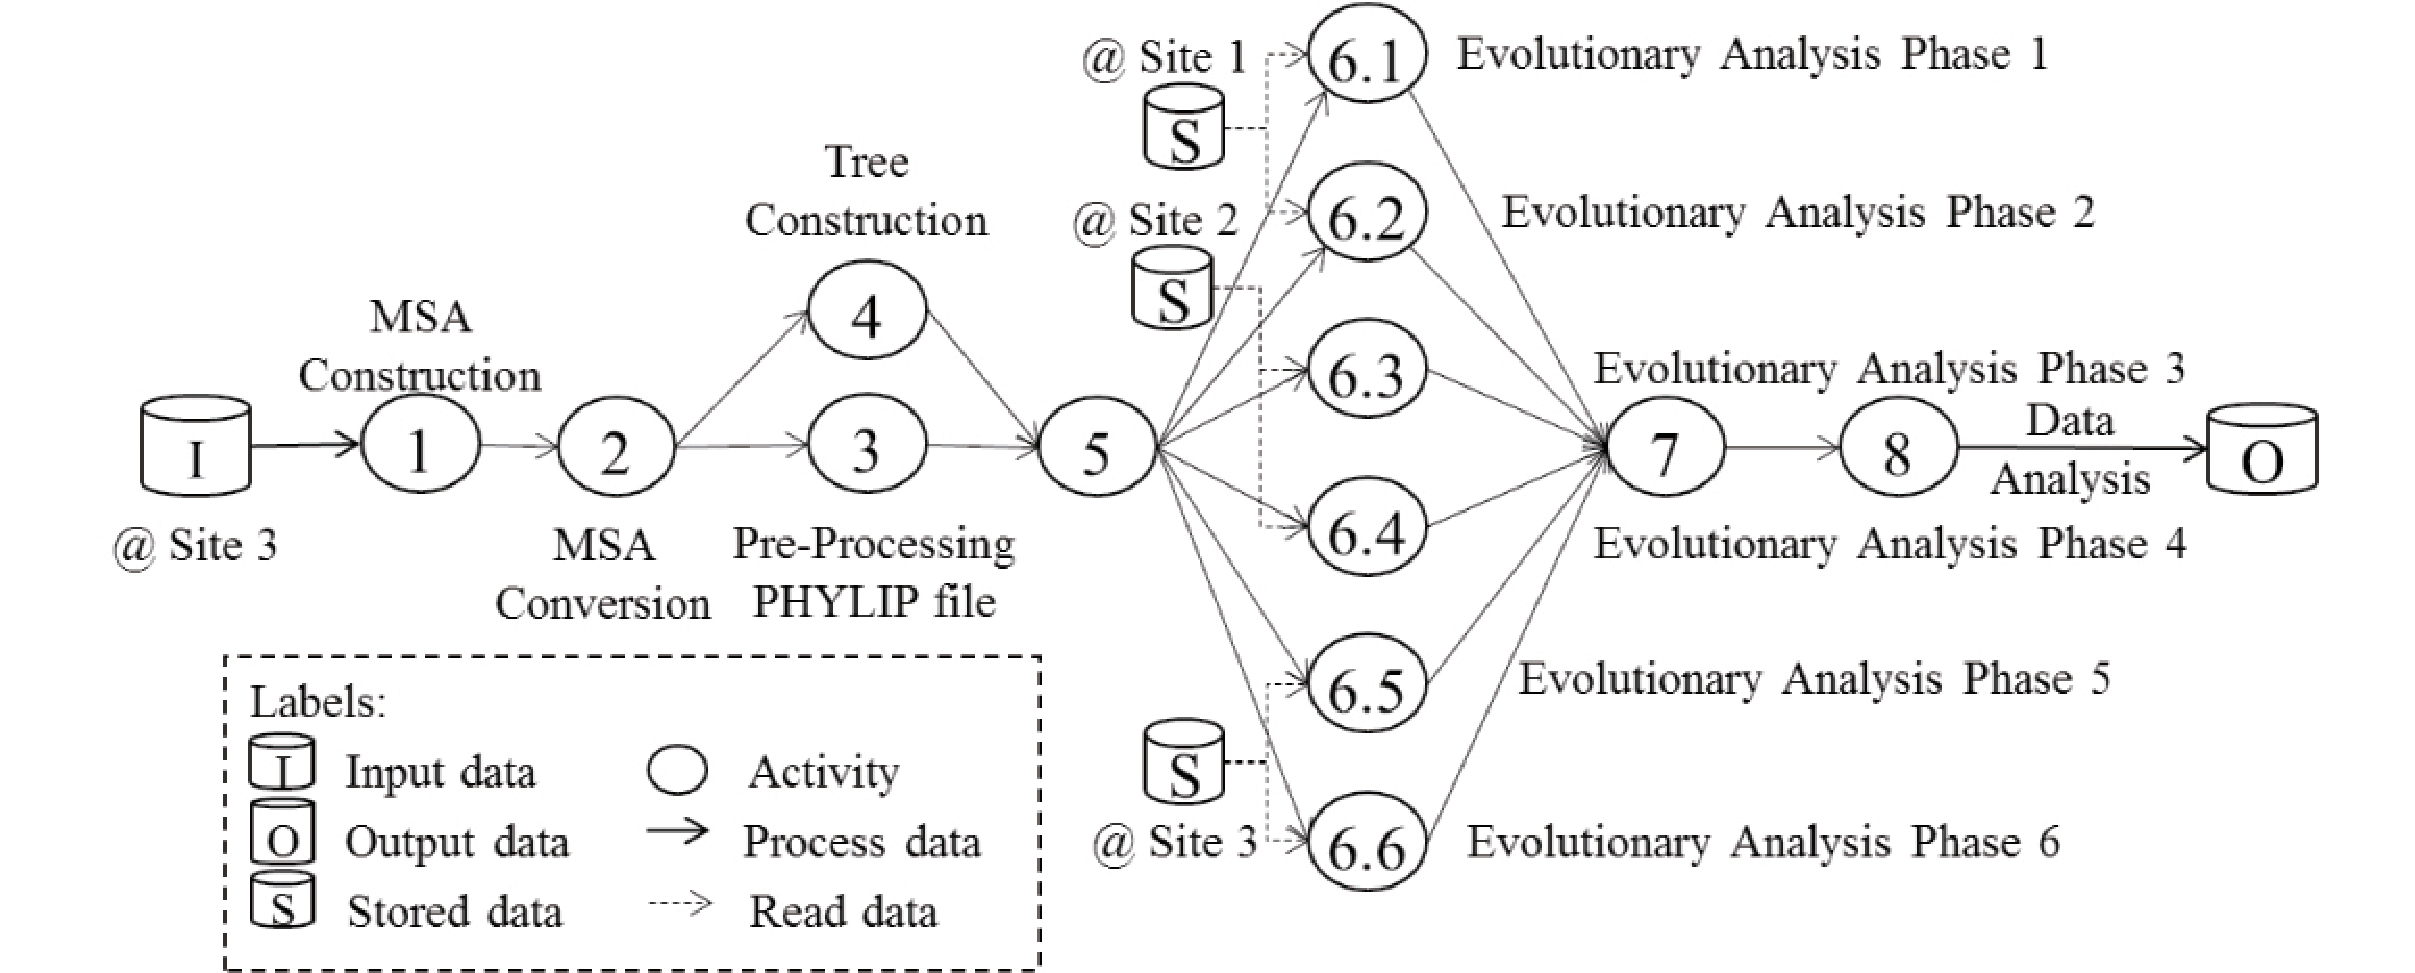
\includegraphics[width=140mm]{figures/FIG2}
\par\end{centering}
\caption{\textbf{SciEvol SWf. }}
\label{fig:scievol}
\end{figure*}

In this section, in order to illustrate partitioning and scheduling approaches, we use the SciEvol SWf use case presented in Chapter \ref{State} with stored data at different cloud sites.
In Figure \ref{fig:scievol}, \enquote{read data} represents that one activity just reads the stored data without modifying it and that the activity should be executed at the corresponding site to read data since the stored data is too big to be moved and can be 
accessed only within the corresponding site because of configurations, \textit{e.g.} security configuration of a database. The stored data constraints are defined by the following matrix (the activities not listed in the matrix are not fixed).

$
\begin{matrix}
 & s_1 & s_2 & s_3 \\
 a_{6.1} &  1 & 0 & 0 \\
 a_{6.2} & 1 & 0 & 0 \\
 a_{6.3} & 0 & 1 & 0 \\
 a_{6.4} & 0 & 1 & 0 \\
 a_{6.5} & 0 & 0 & 1 \\
 a_{6.6} & 0 & 0 & 1 \\
\end{matrix}
$


\subsection{Scheduling approaches}

In this section, we propose three multisite scheduling algorithms. The first one, \textit{LocBased} is adapted from the scheduling algorithm used in Chapter \ref{SWPMC}, which schedules a fragment to the site that stores the data while reducing data transfer among different sites. The second one, \textit{SGreedy}, is adapted from the greedy scheduling algorithm designed for multi-objective single site scheduling in our previous work \cite{Oliveira2012}, which schedules the most suitable fragment to each site. The last one, \textit{ActGreedy}, which combines characteristics of the two adapted algorithms, schedules the most suitable site to each fragment. In addition, we propose that a fixed activity can only be scheduled and executed at the site where the stored data is located. This is applied by analyzing the constraint matrix in all the three algorithms before other steps, which are not explicitly presented in the algorithms.
\begin{figure}[htbp]
\begin{centering}
\captionsetup{justification=centering}
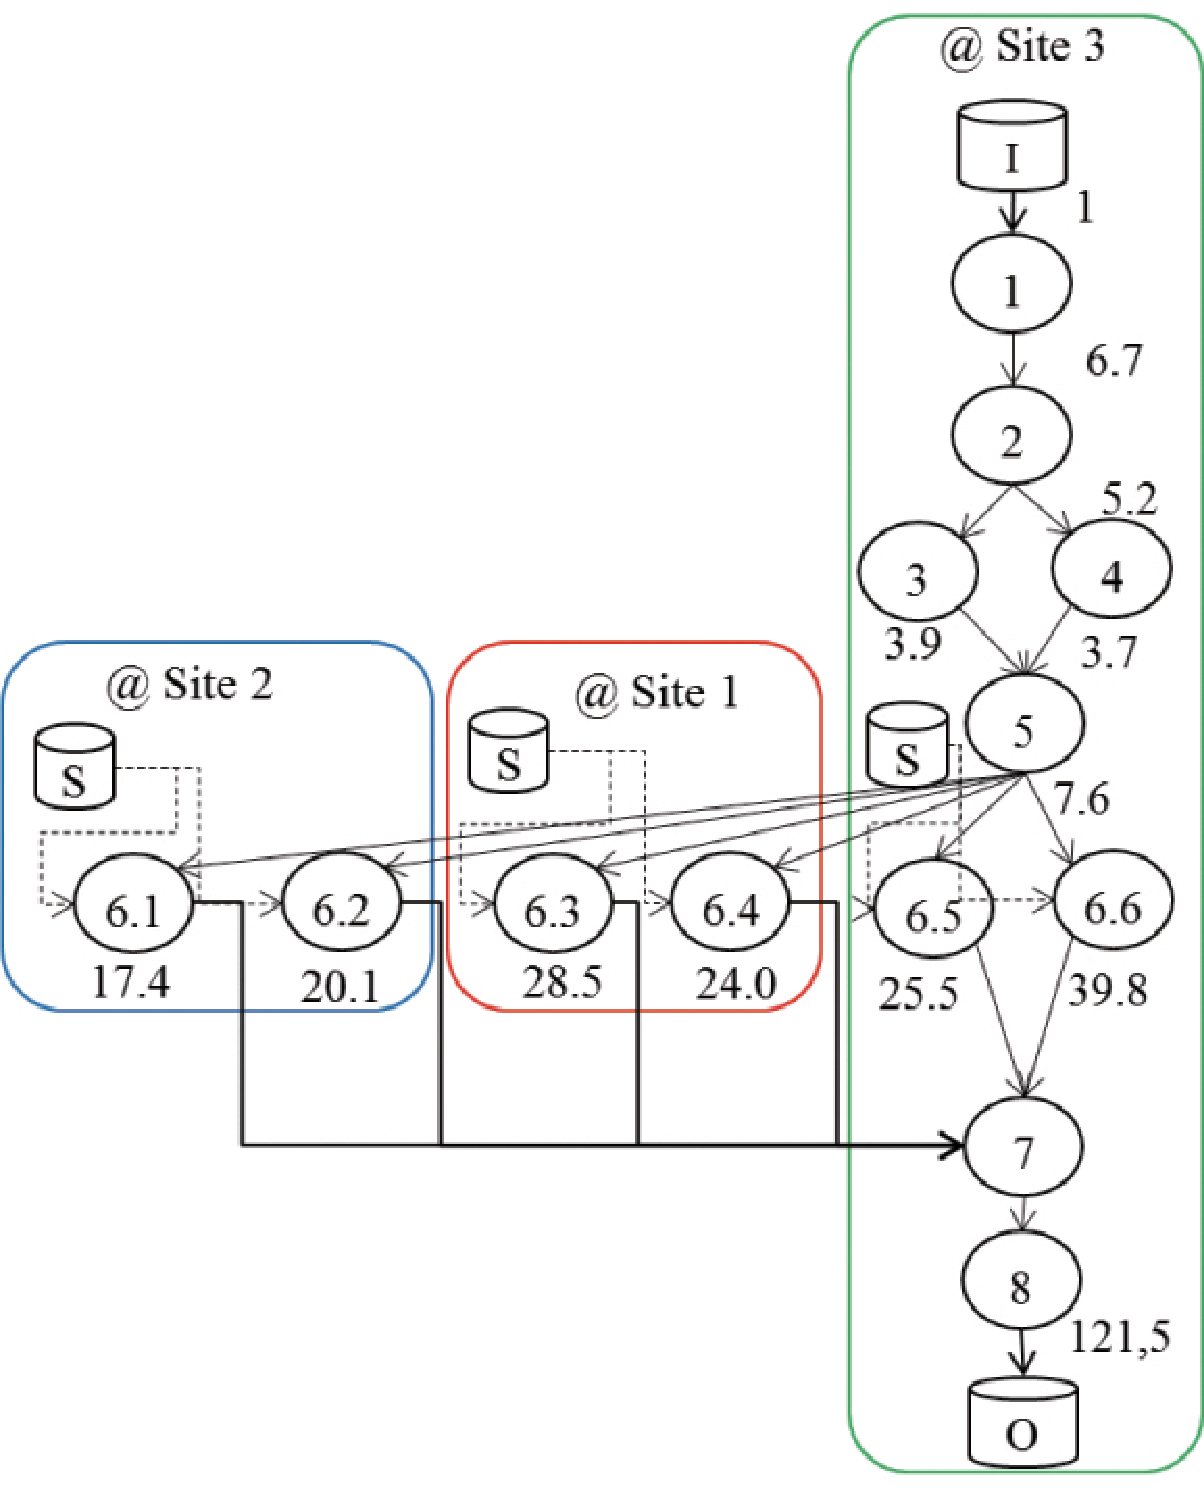
\includegraphics[width=90mm]{figures/FIG3}
\par\end{centering}
\caption{\textbf{SWf partitioning and data location based scheduling.} The number represents the relative (compared with the input data) amount of output data for corresponding activities.}
\label{fig:LocBased}
\end{figure}

\subsubsection{Data Location Based Scheduling}

We adapt the scheduling approach proposed in \cite{Liu2014} to the multisite cloud environment. Since this approach is based on the location of data, we call it LocBased (data location based) scheduling, which is given in Algorithm \ref{alg:LocBased}. Line $2$ partitions a Fragment $wf$ using the data transfer minimization algorithm (Algorithm \ref{alg:wp} in Section \ref{sec:WPT}) as shown in Figure \ref{fig:LocBased}. Then, each fragment $wf$ (Line $3$) is scheduled to a data site (Line $4-5$). If the fragment contains a fixed activity, the scheduled data site is the site that stores the required data (\textit{i.e.} stored data) of the fixed activity. If the fragment does not contain a fixed activity, the scheduled data site is the site that stores the biggest part of the input data of the fragment.

Algorithm \ref{alg:LocBased} schedules the fragment to the data site that stores the required data (\textit{i.e.} stored data for fixed activity) or the biggest part of the input data (for normal activities) in order to reduce the time and monetary costs to transfer data among different sites. However, the granularity of this scheduling algorithm is relatively big and some activities are scheduled at a site that incurs high cost. For instance, the result of this algorithm is shown in Figure \ref{fig:LocBased} while Activity $1, 2, 3, 4, 5, 7$ and $8$ can be scheduled at Site $1$, which is less expensive to use VMs than at other sites.

\begin{algorithm}
\caption{Data location based scheduling}\label{alg:LocBased}
\begin{algorithmic}[1]
\INPUT $swf$: a scientific workflow; $S$: a set of sites
\OUTPUT $SP$: scheduling plan for $swf$ in $S$
\State $SP\gets \emptyset$
\State $WF\gets partition( WF )$ \Comment{According to Algorithm \ref{alg:wp}}
\ForAll{ $wf_i\in WF$ }
\State 	$s_j\gets GetDataSite( wf_i, S )$ \Comment{get Site $s_j$ that stores its required data or the biggest amount of input data}
\State	$SP \gets SP \bigcup \{ Schedule( wf_i , s_j ) \}$
\EndFor
\ENDBEGIN
\end{algorithmic}
\end{algorithm}

\subsubsection{Site Greedy Scheduling}
\label{sec:SGS}

\begin{algorithm}
\caption{Site greedy scheduling}\label{alg:greedy}
\begin{algorithmic}[1]
\INPUT $swf$: a scientific workflow; $S$: a set of sites
\OUTPUT $SP$: scheduling plan for $swf$ in $S$
\State $SP\gets \emptyset$
\State $WF\gets partition( WF )$ \Comment{According to activity encapsulation partitioning method}
\While{$WF \neq \emptyset$}
\ForAll{$s \in S$}
\State $WFA\gets GetAvailableFragments(WF)$ 
\If{$WFA \neq \emptyset$}
\ForAll{$wf \in WFA$}
\State $Cost[i]\gets EstimateCost( wf, s )$ \Comment{According to the cost estimation method}
\EndFor
\State $wf_{opt} \gets GetFragment( s, Cost )$ \Comment{Get the fragment that takes the minimal cost for the execution at Site $s$}
\State $SP \gets SP \bigcup \{ Schedule(wf_{opt},s)\}$
\State $WF \gets WF - wf_{opt}$
\State $WFA \gets GetAvailableFragments(WF)$
\EndIf
\EndFor
\EndWhile
\ENDBEGIN
\end{algorithmic}
\end{algorithm}

We adapt a Site Greedy (SGreedy) scheduling algorithm proposed by de Oliveira \textit{et al.} \cite{Oliveira2012}, for multiple objectives in a multisite environment. Algorithm \ref{alg:greedy} describes SGreedy. When there is a fragment that is not scheduled (Line $3$), for each site (Line $4$), the fragment that takes the least cost is scheduled to each site (Line $5 - 10$). The fragments are selected from the available fragments (Line $5$ and $12$). Line $7-8$ estimate the total cost to execute Fragment $wf$ at the site. Line $9$ chooses the optimal fragment, \textit{i.e.} $wf_{opt}$, that needs the smallest total cost to be executed for the site. Line $10$ schedules the optimal fragment to the site. Line $11$ updates the fragments that need to be scheduled. Line $12$ prepares available fragments to be scheduled for the next site.

This algorithm intends to keep all the sites busy and chooses the best fragment for each site. However, as shown in Figure \ref{fig:SGreedy}, this algorithm may break the dataflow between the parent activity and child activity, which may incur high cost to transfer the data among different sites, \textit{e.g.} Activities $1, 2, 3, 4, 7, 8$. In addition, in order to avoid useless usage of VMs at Site $1$ and Site $2$ during the execution of the SWf, the VMs are shut down after finishing the execution of the corresponding activities, and restarted for the following activities when the input data is ready. After executing Activities $1$, $6.3$ and $6.4$, the VMs at Site $1$ are shut down. The VMs at Site $2$ are shut down after executing Activity $2$. Since Activity $5$ is a control activity, which takes little time to be executed, the VMs at Site $1$ and $3$ are not shut down after executing Activities $4$ and $3$. When the execution of Activities $6.5$ and $6.6$ are to be finished, the VMs at Site $2$ are restarted to continue the execution (since the execution of Activities $6.5$ and $6.6$ may take more time because of big workload). This process may also incur high cost when there are many VMs to restart.

\begin{figure}
\begin{centering}
\captionsetup{justification=centering}
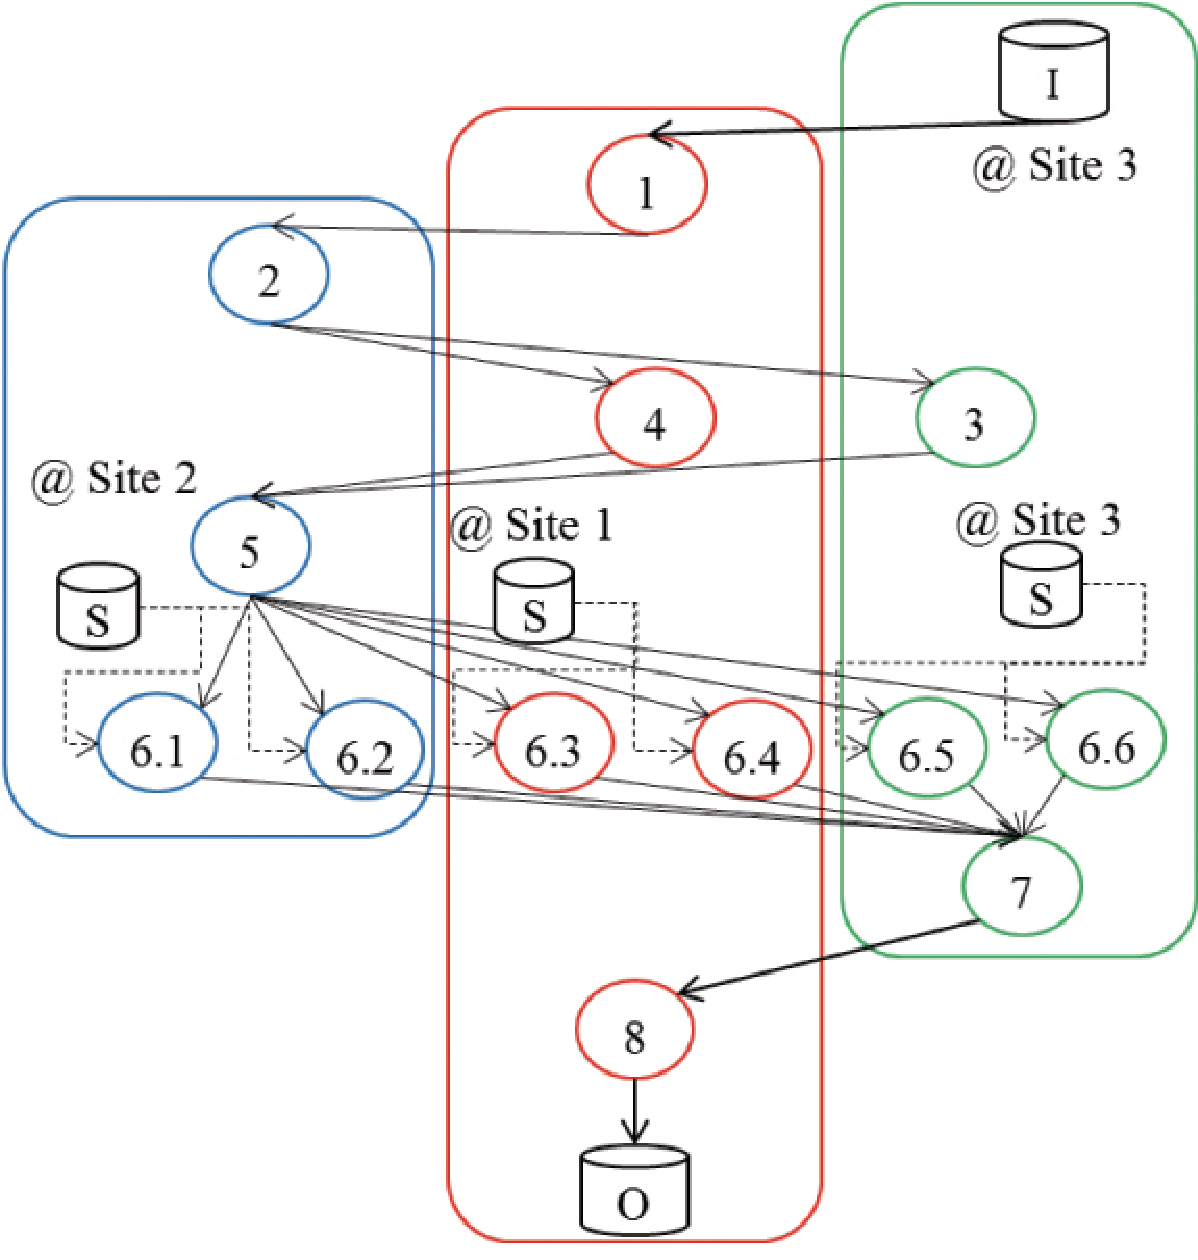
\includegraphics[width=90mm]{figures/FIG4}
\par\end{centering}
\caption{\textbf{Site greedy scheduling.}}
\label{fig:SGreedy}
\end{figure}

\subsubsection{Activity Greedy Scheduling}

\begin{algorithm}[ht]
\caption{Activity greedy scheduling}\label{alg:ActGreedy}
\begin{algorithmic}[1]
\INPUT $swf$: a scientific workflow; $S$: a set of sites
\OUTPUT $SP$: scheduling plan for $swf$ in $S$
\State $SP\gets \emptyset$
\State $SWfCost \gets \infty$
\State $WF\gets partition( swf )$ 
\Do
\State $SP' \gets \emptyset$
\State $WF\gets Group(WF)$ 
\Do
\State $WFA \gets GetAvailableFragments(WF, SP')$
\If{$WFA \neq \emptyset$}
\ForAll{$wf\in WFA$}
\State $s_{opt} \gets BestSite( wf, S )$ 
\State $SP' \gets SP' \bigcup \{Schedule( wf, s_{opt} )\}$
\State update $CurrentSWfCost$
\EndFor
\EndIf
\doWhile{not all the fragments $\in WF$ are scheduled}
\If{$CurrentSWfCost < SWfCost$}
\State $SP \gets SP'$
\State $SWfCost \gets CurrentSWfCost$
\EndIf
\doWhile{$CurrentSWfCost < SWfCost$}
\ENDBEGIN
\end{algorithmic}
\end{algorithm}

Based on LocBased and SGreedy, we propose the ActGreedy (Activity Greedy) scheduling algorithm, which is described in Algorithm \ref{alg:ActGreedy}. 
In this algorithm, all the fragments of a SWf are not scheduled, \textit{i.e.} $Sch(SWf, S) = \emptyset$, at beginning. During the scheduling process, all the fragments are scheduled at a corresponding site, which takes the minimum cost, namely $Sch(SWf, S) = \{ Schedule(wf, s)| wf \in SWf, s \in S\}$ and $\forall ~wf \in SWf, \exists ~Schedule(wf, s) \in Sch(SWf, S)$ while cost $Cost(Schedule(wf, s))$ is the minimum compared to schedule Fragment $wf$ to other sites. As a result, the cost $Cost(Sch(SWf, S))$ of executing a SWf in a multisite cloud is minimized.
Similar to LocBased, ActGreedy schedules fragments of multiple activities. ActGreedy can schedule a pipeline of activities to reduce data transfer between different fragments, \textit{i.e.} the possible data transfer between different sites. As formally defined in \cite{Rodriguez2015}, a pipeline is a group of activities with a one-to-one, sequential relationship between them. However, ActGreedy is different from LocBased since it makes a trade-off between time and monetary costs. Similar to SGreedy, ActGreedy schedules the available fragments, while choosing the best site for an available fragment instead of choosing the best fragment for an available site.

ActGreedy chooses the best site for each fragment. 
First, it partitions a SWf according to the activity encapsulation partitioning method (Line $3$). 
Then, it groups the fragments of three types into bigger fragments to be scheduled (Line $6$).
The first type is a pipeline of activities. We use a recursive algorithm presented in \cite{Rodriguez2015} to find pipelines. Then, the fragments of corresponding activities of each pipeline are grouped into a fragment.
If there are stored activities of different sites in a fragment of a pipeline, the fragment is partitioned into several fragments by the data transfer minimization algorithm (Algorithm \ref{alg:wp}) in the $Group$ function.
The second type is the control activities. If it has only one preceding activity, a control activity is grouped into the fragment of its preceding activity. If it has multiple preceding activities and only one following activity, a control activity (Activity $7$) is grouped into the fragment of its following activity (Activity $8$). If it has multiple preceding activities and multiple following activities, a control activity (Activity $5$) is grouped into the fragment of one of its preceding activities (Activity $3$), which has the most data dependencies among all its preceding activities, \textit{i.e.} the amount of data to be transferred in the data dependency is the biggest.
It reduces data transfer among different fragments, namely the data transfer among different sites, to group the fragments for pipelines and control activities.
The third type is the activities that are scheduled at the same site and that they have dependencies to connect each activity of them.
Afterwards, Line $8$ gets the available fragments (see Section \ref{subsec:CE}) to be scheduled to the best site (Line $11 - 12$), which takes the minimal cost among all the sites to execute the fragment. The cost is estimated according to the method presented in Section \ref{subsec:CE}. When estimating the cost, if the scheduled fragment has data dependencies with fixed activities, the cost to transfer the data in these data dependencies will be taken into consideration. The loop (Lines $7-14$) schedules each fragment to the best site while the big loop (Lines $4 - 18$) improves the scheduling plans by rescheduling the fragments after grouping the fragments at the same site, which ensures that the final scheduling plan corresponds to smaller cost to execute a SWf.

As shown in Figure \ref{fig:ActGreedy}, this algorithm has relatively small granularity compared with LocBased. ActGreedy exploits data location information to select the best site in order to make a trade-off between the cost for transferring data among different sites and another cost, \textit{i.e.} the cost to provision the VMs and the cost to execute fragments. Figure \ref{fig:ActGreedy} shows the scheduling result. If the amount of data increases and the desired execution time is small, Activity $7$ and Activity $8$ may be scheduled at Site $3$, which takes less cost to transfer data. In order to avoid useless usage of VMs, the VMs at Site $1$ are shut down when the site is waiting for the output data of the execution of Site $3$, namely the execution of Activity $6.5$ and Activity $6.6$.


\begin{figure}[htbp]
\begin{centering}
\captionsetup{justification=centering}
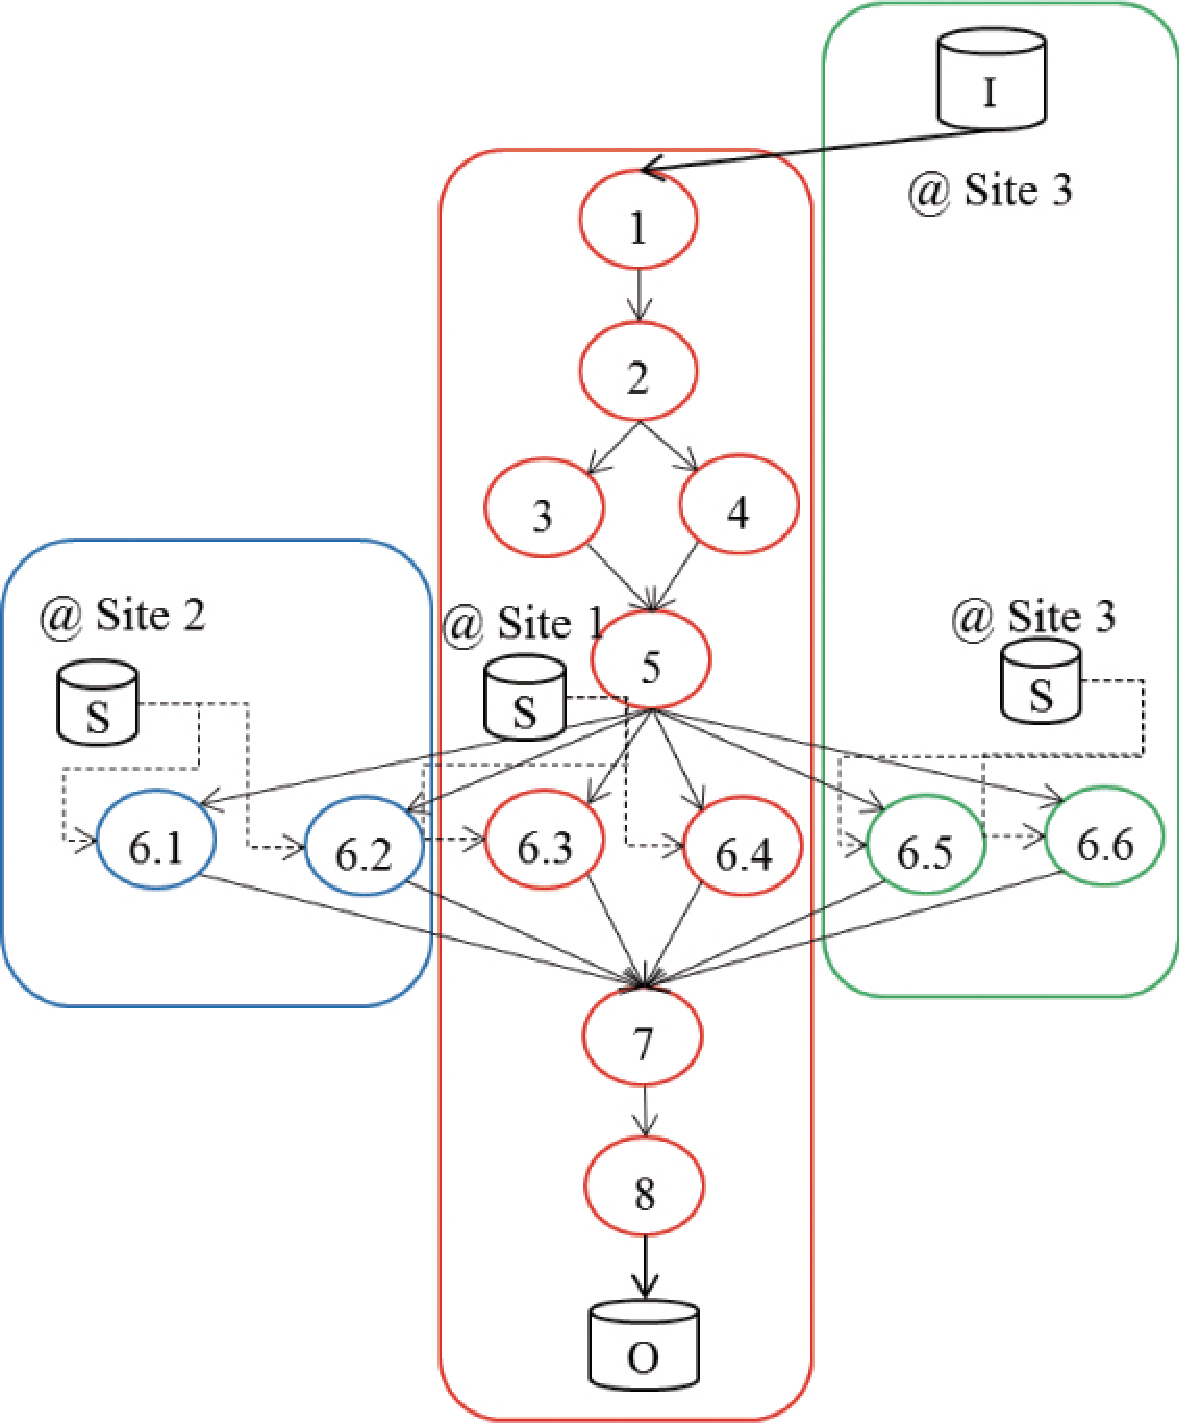
\includegraphics[width=90mm]{figures/FIG5}
\par\end{centering}
\caption{\textbf{Activity greedy scheduling.}}
\label{fig:ActGreedy}
\end{figure}

\subsubsection{Solution analysis}

\begin{table*}[htbp]
\caption{\textbf{Parameters of different types of VMs. } Type represents the type of VMs. vCPUs represents the number of virtual CPUs in a VM. RAM represents the size of memory in a VM. Disk represents the size of hard disk in a VM. CC represents the computing capacity of VMs. MC represents Monetary Cost.} 
\label{tab:VMP}
\begin{centering}
\captionsetup{justification=centering}
\begin{tabular}{|c|c|c|c|c|c|c|c|}
\hline 
Type & vCPUs & RAM & Disk & CC & MC @ WE & MC @ JW & MC @ JE \tabularnewline
\hline 
A1 & 1 & 1.75 & 70 & 9.6 & 0.0447 & 0.0544 & 0.0604 \tabularnewline
A2 & 2 & 3.5 & 135 & 19.2 & 0.0894 & 0.1088 & 0.1208\tabularnewline
A3 & 4 & 7 & 285 & 38.4 & 0.1788 & 0.2176 & 0.2416 \tabularnewline
A4 & 8 & 14 & 605 & 76.8 & 0.3576 & 0.4352 & 0.4832 \tabularnewline
\hline 
\end{tabular}
\par\end{centering} 
\end{table*}

Let us assume that we have $n$ activities, $s$ cloud sites and $f$ fixed activities. The solution search space of a general scheduling problem is $\mathcal{O}(s^n)$. The solution search space of a scheduling problem after fixing the activities becomes $\mathcal{O}(s ^ { n - f })$. Even though the search space is reduced because of \textit{stored data constraints}, the problem remains hard since the search space exponentially increases when $n$ becomes bigger. For instance, assuming that we have a SWf with $77$ activities ($6$ fixed activities) to be schedule at $3$ sites, the search space of a general scheduling problem is $\mathcal{O}(3^{77})$, \textit{i.e.} $\mathcal{O}(5.47 * 10^{36})$, and that of the scheduling problem with fixed activities is $\mathcal{O}(3^{71})$, \textit{i.e.} $\mathcal{O}(7.51 * 10^{33})$. Some input or output activities may be related to the fixed activities, but they are free to be scheduled at any site. In general, the number of fixed activities is quite small compared with the number of other activities. The complexity of our proposed algorithm (ActGreedy) is $\mathcal{O}(s * ( n - f ))$, which is much smaller than $\mathcal{O}(s ^ { n - f })$. As a result, our solution can resolve the problem within reasonable scheduling time, \textit{i.e.} the time to generate scheduling plans.

The knowledge of the location of stored data can be obtained by the metadata of files stored at each site, which is easy to get before SWf execution. Then, the knowledge of fixed activities can be generated with the dependencies between activities and data. Thus, knowing fixed activities is not a problem. 

Our solution generates a scheduling plan that corresponds to the minimum cost to execute a SWf in a multisite cloud since all the fragments are scheduled to a site, which takes the minimum  or near-minimum cost to execute them. The fragments of small granularity are scheduled to the best site, which takes the minimum cost to execute the fragments, by the small loop (Lines $7 - 14$) while the scheduling of fragments of big granularity, \textit{i.e.} the activities of a site, is ensured by big loop (Lines $4-18$). Thus, our proposed algorithm can generate a scheduling plan which may minimize the cost. Since the weight of each objective is positive and the generated scheduling plan may minimize the sum function of multiple objectives, the solution may also be Pareto optimal \cite{Zadeh1963} \cite{Marler2004}. Although, in some rare cases, \textit{e.g.} the cost to transfer data between different sites affects the scheduling plans, the cost corresponding to the generated scheduling plan is not minimum, our proposed solution generates a near-optimal scheduling plan. Since the experiments presented in this chapter are not rare cases, and that the scheduling plan generated by our algorithm is already Pareto optimal (no better scheduling plan can be found by estimating the cost of other scheduling plans), we do not compare it with another optimal solution, which may not even exist.

Note that the proposed algorithm and the results shown in Section \ref{sec:Val} are sensitive to the cost model. Although the cost model is mentioned in other work \cite{Oliveira2012}, it is not used in a multisite environment with stored data constraints. 


\section{Experimental Evaluation}
\label{sec:Val}

\begin{table}[htbp]
\caption{\textbf{Estimated amount of data transferred in a dependency. } Input data represents the number of input fasta files for executing SciEvol SWf.} 
\label{app:DE}
\begin{centering}
\captionsetup{justification=centering}
\begin{tabular}{|c|c|c|c|}
\hline 
\multirow{ 3}{*}{Dependency} & \multicolumn{3}{|c|}{Number of Fasta Files} \\
\cline{2-4}
& $100$ & $500$ & $1000$ \\
\cline{2-4}
& \multicolumn{3}{|c|}{Estimated Amount of Data} \tabularnewline
\hline
Input Data & $1$ & $5$ & $10$ \tabularnewline
$e_{1,2}$ & $6$ & $32$ & $67$ \tabularnewline
$e_{2,3}$ & $5$ & $24$ & $52$ \tabularnewline
$e_{3,5}$ & $3$ & $17$ & $39$ \tabularnewline
$e_{4,5}$ & $3$ & $16$ & $37$ \tabularnewline
$e_{5,6.1}$ & $6$ & $33$ & $76$ \tabularnewline
$e_{6.1,7}$ & $16$ & $85$ & $174$ \tabularnewline
$e_{6.2,7}$ & $20$ & $100$ & $201$ \tabularnewline
$e_{6.3,7}$ & $28$ & $140$ & $285$ \tabularnewline
$e_{6.4,7}$ & $23$ & $118$ & $240$ \tabularnewline
$e_{6.5,7}$ & $24$ & $125$ & $255$ \tabularnewline
$e_{6.6,7}$ & $34$ & $175$ & $348$ \tabularnewline
$e_{7,8}$ & $120$ & $605$ & $1215$ \tabularnewline
\hline 
\end{tabular}
\par\end{centering} 
\end{table}

In this section, we present an experimental evaluation of the fragment scheduling algorithms. 
All experiments are based on the execution of the SciEvol SWf in Microsoft Azure multisite cloud.
We compare ActGreedy with LocBased and SGreedy, as well as with two general algorithms, \textit{i.e.} Genetic and Brute-force.
In the experiments, we consider three Azure \cite{Azure} sites to execute SciEvol SWf, namely West Europe as Site $1$, Japan West as Site $2$, Japan East as Site $3$.
During the experiments, the the life circle of VM is composed of creation, start, configuration, stop and deletion. The creation, start, stop and deletion of a VM is managed by using Azure CLI. The configuration of VM is realized by Linux SSH command.
In the experiments, workflow partitioner, multisite scheduler and single site initialization are simulated, but the execution of fragments is performed in a real environment by Chiron \cite{Ogasawara2013}. 
We conduct the experiments to show that ActGreedy takes the smallest cost (compared with LocBased and SGreedy) to execute a SWf in a multisite cloud within reasonable time (compared with Genetic and Brute-force) by making a trade-off of different objectives based on SSVP. Microsoft Azure provides $5$ tiers of VM, which are basic tier, standard tier, optimized compute, performance optimized compute and compute intensive. Each tier of VM contains several types of VMs. In one Web domain, users can provision different types of VMs at the same tier. In our experiments, we consider $4$ types, namely $A1$, $A2$, $A3$ and $A4$, in the standard tier. The features of the VM types are summarized in Table \ref{tab:VMP}. In Azure, the time quantum is one minute. In addition, the average time to provision a VM is estimated as $2.9$ minutes. Each VM uses Linux Ubuntu 12.04 (64-bit), and is configured with the necessary software for SciEvol. All VMs are configured to be accessed using Secure Shell (SSH).

In the experiments, we use $100$, $500$, $1000$ fasta files generated from the data stored in a genome database \cite{Oma}\cite{OmaGroup}. The programs used are similar to that presented in Section \ref{sec:PVal}. The estimated workload (in GFLOP) of each activity of SciEvol SWf for different numbers of input fasta files is shown in Table \ref{app:pWE}. In Table \ref{app:DE}, $e_{i,j}$ represents the data dependency between Activity $i$ and Activity $j$ while Activity $j$ consumes the output data of Activity $i$. Let DataSize($e_{i,j}$) represent the estimated amount of data in dependency $e_{i,j}$. Then, we have DataSize($e_{2,3}$) = DataSize($e_{2,4}$); DataSize($e_{4,5}$) = DataSize($e_{3,5}$); DataSize($e_{5,6.1}$) = DataSize($e_{5,6.2}$) = DataSize($e_{5,6.3}$) = DataSize($e_{5,6.4}$) = DataSize($e_{5,6.5}$) = DataSize($e_{5,6.6}$).


In the tables and figures, the unit of time is minute, the unit of monetary cost is Euro, the unit of RAM and Disk is Gigabytes, the unit of data is MegaByte (MB), the computing capacity of VMs is GigaFLOPS (GFLOPS) and the unit of workload is GigaFLOP (GFLOP). $\omega_t$ represents the weight of time cost. $A1$, $A2$, $A3$ and $A4$ represent the types of VMs in Azure. [Type of VM] * [number] represents provisioning [number] of VMs of [Type of VM] type, \textit{e.g.} A1 * 1 represents provisioning one VM of A1 type. WE represents West Europe; JW Japan West and JE Japan East. The cost corresponds to the price in Euro of Azure on July 27, 2015.

\begin{table}[htbp]
\caption{\textbf{Setup parameters. } ``Number'' represents the number of input fasta files. ``Limit'' represents the maximal number of virtual CPUs that can be instantiated in the cloud. ``DET'' represents Desired Execution Time and ``DMC'' represents Desired Monetary Cost.}
\label{tab:Set}
\begin{centering}
\captionsetup{justification=centering}
\begin{tabular}{|c|c|c|c|c|}
\hline 
Number & $100$ & $500$ & $1000$ \tabularnewline
\hline 
Limit & $350$ & $350$ & $350$ \tabularnewline
\hline 
Estimated workload & $414,720$ & $3,000,000$ & $6,000,000$\tabularnewline
\hline 
DET & $60$ & $60$ & $60$ \tabularnewline
\hline 
DMC & $0.3$ & $3$ & $6$ \tabularnewline
\hline 
\end{tabular}
\par\end{centering} 
\end{table}

\begin{table}[htbp]
\caption{\textbf{VM Provisioning Plans (100 fasta files). }} 
\label{tab:VMD1}
\begin{centering}
\captionsetup{justification=centering}
\begin{tabular}{|c|c|c|c|c|}
\hline 
\multirow{ 2}{*}{Algorithm} & \multirow{ 2}{*}{Site} & \multicolumn{3}{|c|}{$\omega_t$} \\
\cline{3-5}
& & 0.1 & 0.5 & 0.9 \tabularnewline
\hline 
\multirow{3}{*}{LocBased} & WE & $A3 * 1$ & $A4 * 1$ & $A4 * 2$ \tabularnewline
& JW & $A3 * 1$ & $A4 * 1$ & $A4 * 1$ \tabularnewline
& JE & $A1 * 1, A2 * 1$ & $A4 * 1$ & $A4 * 3$ \tabularnewline
\hline
\multirow{3}{*}{SGreedy} & WE & $A3 * 1$ & $A4 * 1$ & $A4 * 2$ \tabularnewline
& JW & $A2 * 1, A3 * 1$ & $A4 * 1$ & $A4 * 1$ \tabularnewline
& JE & $A1 * 1, A2 * 1$ & $A4 * 1$ & $A4 * 3$ \tabularnewline
\hline 
\multirow{3}{*}{ActGreedy} & WE & $A2 * 1$ & $A2 * 1; A3 * 1$ & $A4 * 2$ \tabularnewline
& JW & $A3 * 1$ & $A4 * 1$ & $A4 * 1$ \tabularnewline
& JE & $A1 * 1, A2 * 1$ & $A4 * 1$ & $A4 * 2$ \tabularnewline
\hline 
\end{tabular}
\par\end{centering} 
\end{table}

\begin{table}[htbp]
\caption{\textbf{VM Provisioning Plans (500 fasta files). }} 
\label{tab:VMD2}
\begin{centering}
\captionsetup{justification=centering}
\begin{tabular}{|c|c|c|c|c|}
\hline 
\multirow{ 2}{*}{Algorithm} & \multirow{ 2}{*}{Site} & \multicolumn{3}{|c|}{$\omega_t$} \\
\cline{3-5}
& & 0.1 & 0.5 & 0.9 \tabularnewline
\hline 
\multirow{3}{*}{LocBased} & WE & $A3 * 1$, $A4 * 1$ & $A4 * 4$ & $A4 * 7$ \tabularnewline
& JW & $A4 * 1$ & $A4 * 2$ & $A4 * 3$ \tabularnewline
& JE & $A1 * 1, A4 * 1$ & $A4 * 3$, $A3 * 1$ & $A4 * 8$ \tabularnewline
\hline
\multirow{3}{*}{SGreedy} & WE & $A3 * 1$, $A4 * 1$ & $A4 * 4$ & $A4 * 7$ \tabularnewline
& JW & $A4 * 1$ & $A4 * 2$ & $A4 * 3$ \tabularnewline
& JE & $A1 * 1, A3 * 1$ & $A3 * 1$, $A4 * 3$ & $A4 * 8$ \tabularnewline
\hline 
\multirow{3}{*}{ActGreedy} & WE & $A4 * 1$ & $A2 * 1; A4 * 2$ & $A4 * 5$ \tabularnewline
& JW & $A4 * 1$ & $A4 * 2$ & $A4 * 3$ \tabularnewline
& JE & $A1 * 1, A4 * 1$ & $A3 * 1$, $A4 * 3$ & $A4 * 9$ \tabularnewline
\hline 
\end{tabular}
\par\end{centering} 
\end{table}

\begin{table}[htbp]
\caption{\textbf{VM Provisioning Plans (1000 fasta files). }} 
\label{tab:VMD3}
\begin{centering}
\captionsetup{justification=centering}
\begin{tabular}{|c|c|c|c|c|}
\hline 
\multirow{ 2}{*}{Algorithm} & \multirow{ 2}{*}{Site} & \multicolumn{3}{|c|}{$\omega_t$} \\
\cline{3-5}
& & 0.1 & 0.5 & 0.9 \tabularnewline
\hline  
\multirow{3}{*}{LocBased} & WE & $A2 * 1$, $A4 * 1$ & $A4 * 6$ & $A4 * 9$ \tabularnewline
& JW & $A4 * 2$ & $A4 * 3$ & $A4 * 4$ \tabularnewline
& JE & $A2 * 1, A3 * 1, A4 * 1$ & $A4 * 5$ & $A4 * 11$ \tabularnewline
\hline
\multirow{3}{*}{SGreedy} & WE & $A4 * 2$ & $A4 * 6$ & $A4 * 10$ \tabularnewline
& JW & $A4 * 2$ & $A4 * 3$ & $A4 * 4$ \tabularnewline
& JE & $A2 * 1, A3 * 1, A4 * 1$ & $A4 * 5$ & $A4 * 11$ \tabularnewline
\hline 
\multirow{3}{*}{ActGreedy} & WE & $A2 * 1, A4 * 1$ & $A4 * 4$ & $A4 * 8$ \tabularnewline
& JW & $A4 * 2$ & $A4 * 3$ & $A4 * 4$ \tabularnewline
& JE & $A2 * 1, A3 * 1, A4 * 1$ & $A4 * 6$ & $A4 * 12$ \tabularnewline
\hline 
\end{tabular}
\par\end{centering} 
\end{table}

We present the experimental results to show that our proposed scheduling algorithm, \textit{i.e.} ActGreedy, leads to the least cost for the execution of SWf in a multisite cloud environment.
We schedule the fixed activities at the site where the data is stored and use the three scheduling algorithms, namely LocBased, SGreedy and ActGreedy, to schedule other activities of SciEvol at the three sites. In addition, we implemented a genetic algorithm and a brute-force algorithm that generate the best scheduling plans similar to those generated by ActGreedy.
Brute-force measures the cost of all the possible scheduling plans and finds the optimal one, corresponding to the minimum cost to execute SWfs in a multisite cloud. The principle of a genetic algorithm \cite{Wieczorek2005} is to encode possible scheduling plans into a population of chromosomes, and subsequently to transform the population using standard operations of selection, crossover and mutation, producing successive generations, until the convergence condition is met. In the experiments, we set the convergence condition so that the cost of scheduling plans should be equal or smaller than that generated by ActGreedy. We use $100$ chromosomes and set the number of generations as $1$ for the experiments of different numbers of input files and different values of $\alpha$. We choose a random point for the crossover and mutation operation. The experimental results\footnote{In the experiments, in order to facilitate the data transfer of many small files, we use the \textit{tar} command to archive the small files into one big file before data transferring.} are shown in Figure \ref{fig:comparision}. The setup parameters are shown in Table \ref{tab:Set} and provisioning plans, which are generated by SSVP, are listed in Table \ref{tab:VMD1}, Table \ref{tab:VMD2} and Table \ref{tab:VMD3}. We assume that the data transfer rate between different sites is $2$ MB/s. The monetary cost to transfer data from Site $1$ to other sites is $0.0734$ Euros/GB and the monetary cost for Site $2$ and Site $3$ is $0.1164$ Euros/GB. In the experiments, the critical path of SciEvol SWf is composed of Activities $1$, $2$, $4$, $5$, $6.6$, $7$, $8$.

\begin{figure*}[htbp]
\begin{centering}
		\subfigure[\textbf{Comparision for 100 fasta files.}]{\includegraphics[width=59mm]{figures/FIG9_1} \label{fig:tc1}} 
		\subfigure[\textbf{Comparision for 500 fasta files.} ]{\includegraphics[width=59mm]{figures/FIG9_2} \label{fig:tc5}}
		\subfigure[\textbf{Comparision for 1000 fasta files.}]{\includegraphics[width=59mm]{figures/FIG9_3} \label{fig:tc10}} 
\caption{\textbf{Cost for different scheduling algorithms.} The cost is calculated according to Formula \ref{eq:eq1}.}\label{fig:comparision}
\end{centering}
\end{figure*} 

LocBased is optimized for reducing data transfer among different sites. The scheduling plan generated by this algorithm is shown in Figure \ref{fig:LocBased}. However, the different monetary costs of the three sites are not taken into consideration. In addition, this algorithm directly schedules a fragment, which contains multiple activities. Some activities are scheduled at a site, which is more expensive to use VMs, \textit{e.g.} Site $3$. As a consequence, the scheduling plan may correspond to higher cost. SGreedy schedules a site to the available activity, which takes the least cost. The corresponding scheduling plan is shown in Figure \ref{fig:SGreedy}. SGreedy does not take data location into consideration and may schedule two continuous activities, \textit{i.e.} one preceding activity and one following activity, to two different sites, which takes time to transfer data and to provision VMs. As a result, this algorithm may lead to higher cost. ActGreedy can schedule each fragment to a site that takes the least cost to execute it, which leads to smaller cost compared with LocBased and SGreedy. In addition, ActGreedy can make adaptive modification for different numbers of input fasta files. For instance, there are three situations where Activity $7$ and Activity $8$ are scheduled at Site $3$ to reduce the cost of data transfer while the other scheduling plans are the same as shown in Figure \ref{fig:ActGreedy}. The three situations are when there are $500$ input fasta files and $\omega_t = 0.9$ and when there are $1000$ input fasta files and $\omega_t = 0.5$ or $\omega_t = 0.9$. Note that SWf partitioning algorithms may also have impact on the performance of the scheduling algorithm. For instance, LocBased is based on a SWf partitioning algorithm to reduce data transfer among different SWf fragments.

\begin{figure}[htbp]
\begin{centering}
\captionsetup{justification=centering}
\includegraphics[width=90mm]{figures/FIG10}
\par\end{centering}
\caption{\textbf{Comparision of cost between SGreedy and ActGreedy for different number of input fasta files.} The cost is calculated according to Formula \ref{eq:eq1}.}
\label{fig:cp}
\end{figure}

First, we analyze the cost based on Formula \ref{eq:eq1} and Formula \ref{eq:eq2}.
The time and monetary costs to execute a fragment at a site are measured during execution. Both the time and monetary costs are composed of three parts, \textit{i.e.} site execution, data transfer and fragment execution. Based on Formulas \ref{eq:eq2}, \ref{eq:eq3}, \ref{eq:eq4}, \ref{eq:eq5}, \ref{eq:eq6}, the cost to execute a fragment is calculated. Based on Formula \ref{eq:eq1} and Formula \ref{eq:eq2}, the cost to execute a SWf is calculated. 
The cost corresponding to $100$ fasta files is shown in Figure \ref{fig:tc1}. In order to execute SciEvol SWf with 100 fasta files, ActGreedy can reduce $1.85$\% ($\omega_t=0.1$), $7.13$\% ($\omega_t=0.5$) and $13.07$\% ($\omega_t=0.9$) of the cost compared with LocBased. Compared with SGreedy, ActGreedy can reduce $3.22$\% ($\omega_t=0.1$), $12.80$\% ($\omega_t=0.5$) and $26.60$\% ($\omega_t=0.9$) of the cost. Figure \ref{fig:tc5} shows the cost for different values of $\omega_t$ for processing $500$ fasta files. The experimental results show that ActGreedy is up to $13.15\%$ ($\omega_t=0.9$) better than LocBased and up to $50.57\%$ ($\omega_t=0.9$) better than SGreedy for $500$ fasta files. In addition, Figure \ref{fig:tc10} shows the experimental results for $1000$ fasta files. The results show that LocBased takes up to $21.75\%$ ($\omega_t=0.1$) higher cost than ActGreedy and that SGreedy takes up to $74.51\%$ ($\omega_t=0.9$) higher cost than ActGreedy when processing $1000$ fasta files. Figure \ref{fig:cp} describes the difference between the worst case (SGreedy) and the best case (ActGreedy). In Figure \ref{fig:cp}, the \textit{Y} axis represents the advantage\footnotemark ~of ActGreedy compared with SGreedy. It can be seen from Figure \ref{fig:cp} that ActGreedy outperforms SGreedy and its advantage becomes obvious when $\omega_t$ grows. When there are more input fasta files, the advantage is bigger at first. But it decreases when the number of fasta files grows from $500$ to $1000$ since the cost corresponding to ActGreedy increases faster.

\footnotetext{The advantage is calculated based on the following formula:
\begin{equation}\label{eq:eq21}
Advanage = \frac{Cost_{SGreedy}(\omega_t) - Cost_{ActGreedy}(\omega_t)} {Cost_{ActGreedy}(\omega_t)} * 100 \%
\end{equation} 
}

\begin{figure*}[htbp]
\begin{centering}
		\subfigure[\textbf{Comparision for 100 fasta files.}]{\includegraphics[width=59mm]{figures/FIG11_1} \label{fig:RC1}} 
		\subfigure[\textbf{Comparision for 500 fasta files.} ]{\includegraphics[width=59mm]{figures/FIG11_2} \label{fig:RC5}}
		\subfigure[\textbf{Comparision for 1000 fasta files.}]{\includegraphics[width=59mm]{figures/FIG11_3} \label{fig:RC10}} 
\caption{\textbf{Cost for different scheduling algorithms.} According to Formula \ref{eq:eq0}.}\label{fig:comparisionRC}
\end{centering}
\end{figure*} 

Accordingly, the cost calculated according to Formula \ref{eq:eq0} is shown in Figure \ref{fig:comparisionRC}. In the real execution, the time and monetary costs for the whole execution of a SWf are measured and the real cost can be calculated by Formula \ref{eq:eq0}. From Figures \ref{fig:RC1}, \ref{fig:RC5} and \ref{fig:RC10}, we can see that the cost corresponding to ActGreedy is smaller than that of SGreedy at all the situations. Except in one situation, ActGreedy performs better than LocBased. When the number of input fasta files is $500$ and $\omega_t=0.5$, the cost for the data transfer becomes important. In this case, LocBased performs slightly better than ActGreedy. However, the advantage of LocBased ($0.03\%$) is very small and this may be because of the dynamic changing environment in the Cloud. As the number of input fasta files increases, the advantage of ActGreedy becomes obvious. Compared with LocBased, ActGreedy is up to $4.1\%$ (100 fasta files and $\omega_t = 0.9$), $7.4\%$ (500 fasta files and $\omega_t = 0.9$) and $10.7\%$ (1000 fasta files and $\omega_t = 0.1$) better. Compared with SGreedy, the advantage of ActGreedy can be up to $7.5\%$ (100 fasta files and $\omega_t = 0.5$), $17.2\%$ (500 fasta files and $\omega_t = 0.9$) and $8.8\%$ (1000 fasta files and $\omega_t = 0.5$).

\begin{figure*}[htbp]
\begin{centering}
		\subfigure[\textbf{Execution time (100 fasta files).}]{\includegraphics[width=59mm]{figures/FIG12_1} \label{fig:ET1}} 
		\subfigure[\textbf{Execution time (500 fasta files).} ]{\includegraphics[width=59mm]{figures/FIG12_2} \label{fig:ET5}}
		\subfigure[\textbf{Execution time (1000 fasta files).}]{\includegraphics[width=59mm]{figures/FIG12_3} \label{fig:ET10}} 
\caption{\textbf{Execution time of SciEvol with different scheduling approaches.}}\label{fig:MOET}
\end{centering}
\end{figure*}

Figures \ref{fig:MOET} and \ref{fig:MC} show the execution time and the monetary costs for the execution of SciEvol with different amounts of input data and different values of $\omega_t$. When $\omega_t$ increases, the execution time is largely reduced and the monetary cost increases. When the weight of execution time cost is low, \textit{i.e.} $\omega_t = 0.1$, Compared with LocBased and SGreedy, ActGreedy may correspond to more execution time while it generally takes less monetary cost. When the weight of execution time cost is high, \textit{$\omega_t = 0.9$}, ActGreedy corresponds to less execution time. The execution with ActGreedy always takes less monetary cost compared with LocBased (up to $14.12\%$) and SGreedy (up to $17.28\%$). The reason is that ActGreedy can choose a cheap site to execute fragments, namely the monetary cost to instantiate VMs at that site is low. As a result, ActGreedy makes a good trade-off between execution time and monetary costs for the execution of SciEvol at a multisite cloud.

Furthermore, we measured the amount of data transferred among different sites, which is shown in Figure \ref{fig:DT}. Since LocBased is optimized for minimizing data transferred between different sites, the amount of intersite transferred data with LocBased remains 
\begin{figure*}[htbp]
\begin{centering}
		\subfigure[\textbf{Monetary cost (100 fasta files).}]{\includegraphics[width=59mm]{figures/FIG13_1} \label{fig:MC1}} 
		\subfigure[\textbf{Monetary cost (500 fasta files).} ]{\includegraphics[width=59mm]{figures/FIG13_2} \label{fig:MC5}}
		\subfigure[\textbf{Monetary cost (1000 fasta files).}]{\includegraphics[width=59mm]{figures/FIG13_3} \label{fig:MC10}} 
\caption{\textbf{Monetary cost of SciEvol execution with different scheduling approaches.}}\label{fig:MC}
\end{centering}
\end{figure*}
\noindent minimum when the number of input fasta files varies from $100$ to $1000$. The amount of transferred data corresponding to ActGreedy is slightly bigger than that of LocBased and the difference is between $1.0\%$ and $13.4\%$. SGreedy has the biggest amount of intersite transferred data. Compared with ActGreedy, the amount of intersite transferred data of SGreedy is up to $122.5\%$, $139.2\%$ and $148.1\%$ bigger when the number of input fasta files is $10$, $500$ and $1000$. In addition, the amount of data transfer with ActGreedy decreases for the three cases, \textit{i.e.} $500$ input fasta files with $\omega_t = 0.9$ and $1000$ input fasta files with $\omega_t = 0.5$ or $\omega_t = 0.9$. The reason is that Activities $7$ and $8$ are scheduled at the same site as Activities $6.5$ and $6.6$, namely Site $3$, which reduces data transfer. Furthermore, when the data transfer rate between different sites decreases, the performance of SGreedy will be much worse since the time to transfer big amounts of data will be much longer. 

In addition, we measure the idleness of the virtual CPUs according to following formula:
\begin{equation}\label{eq:eq22}
Idleness = \frac{\sum_{i=1}^{n}IdleTime(CPU_i)} {\sum_{i=1}^{n}TotalTime(CPU_i)} * 100 \%
\end{equation} 
where $n$ represents the number of virtual CPUs, $IdleTime$ represents the time when the virtual CPU is not working for the execution of the programs of SciEvol SWf. $TotalTime$ represents the total time that the virtual CPU is instantiated. 


Figure \ref{fig:idleness} shows the idleness of virtual CPUs corresponding to different scheduling algorithms and different amounts of fasta files. From the figure, we can see that as $\omega_t$ increases, the idleness becomes bigger. When $\omega_t$ increases, the importance of execution time becomes bigger and more VMs are provisioned to execute fragments. 
\begin{figure*}[htbp]
\begin{centering}
		\subfigure[\textbf{Intersite data transfer ($\omega_t = 0.1$).}]{\includegraphics[width=59mm]{figures/FIG14_1} \label{fig:DT1}} 
		\subfigure[\textbf{Intersite data transfer ($\omega_t = 0.5$).} ]{\includegraphics[width=59mm]{figures/FIG14_2} \label{fig:DT5}}
		\subfigure[\textbf{Intersite data transfer ($\omega_t = 0.9$).}]{\includegraphics[width=59mm]{figures/FIG14_3} \label{fig:DT9}} 
\caption{\textbf{Intersite data transfer for different scheduling algorithms.}}\label{fig:DT}
\end{centering}
\end{figure*}
In this case, the time to start the VMs becomes higher compared with execution time. As a result, the corresponding idleness goes up. In addition, when the amount of input files, \textit{i.e.} fasta files, rises, the idleness decreases. The reason is that at this situation, more time is used for the execution of SWf for the increased workload. The figure also shows that LocBased has the smallest idleness while SGreedy has the biggest idleness. This is expected since the VMs at Sites $1$ and $2$ need to be shut down and restarted during the execution with SGreedy and that the VMs at Site $1$ needs to be shut down and restarted during the execution with ActGreedy. The time to restart VMs at a site may consume several minutes while the virtual CPUs are not used for the execution of fragments. Figure \ref{fig:idle1}, Figure \ref{fig:idle5} and Figure \ref{fig:idle5} show the experimental results for the corresponding idleness of virtual CPUs. From the figures, we can see that the idleness of ActGreedy is generally bigger than that of LocBased while it is always smaller than that of SGreedy. The idleness of ActGreedy is up to $38.2\%$ ($\omega_t = 0.5$) bigger than that of LocBased and up to $37.8\%$ ($\omega_t = 0.1$) smaller than that of SGreedy for $100$ fasta files. The idleness of ActGreedy is up to $12.4\%$ ($\omega_t = 0.1$) bigger than that of LocBased and up to $38.0\%$ ($\omega_t = 0.5$) smaller than that of SGreedy for $500$ fasta files. For $1000$ fasta files, the idleness of ActGreedy is $18.6\%$ ($\omega_t = 0.1$) and $1.0\%$ ($\omega_t = 0.9$) bigger than that of LocBased. When $\omega_t = 0.5$, the idleness of ActGreedy is $20.9\%$ smaller than that of LocBased. In addition, the idleness of ActGreedy is up to $50.9\%$ ($\omega_t = 0.5$) smaller than that of SGreedy.
\begin{figure*}
\begin{centering}
		\subfigure[\textbf{Idleness of virtual CPUs for 100 fasta files.}]{\includegraphics[width=59mm]{figures/FIG15_1} \label{fig:idle1}} 
		\subfigure[\textbf{Idleness of virtual CPUs for 500 fasta files.} ]{\includegraphics[width=59mm]{figures/FIG15_2} \label{fig:idle5}}
		\subfigure[\textbf{Idleness of virtual CPUs for 1000 fasta files.}]{\includegraphics[width=59mm]{figures/FIG15_3} \label{fig:idle10}} 
\caption{\textbf{Idleness of virtual CPUs for different scheduling algorithms.} According to Formula \ref{eq:eq22}.}\label{fig:idleness}
\end{centering}
\end{figure*}

Finally, we study the scheduling time of different algorithms. In order to show the effectiveness of ActGreedy, we compare it with our two other algorithms, \textit{i.e.} SGreedy and LocBased, and two more general algorithms, \textit{i.e.} Genetic and Brute-force. 

\begin{figure*}
\begin{centering}
\captionsetup{justification=centering}
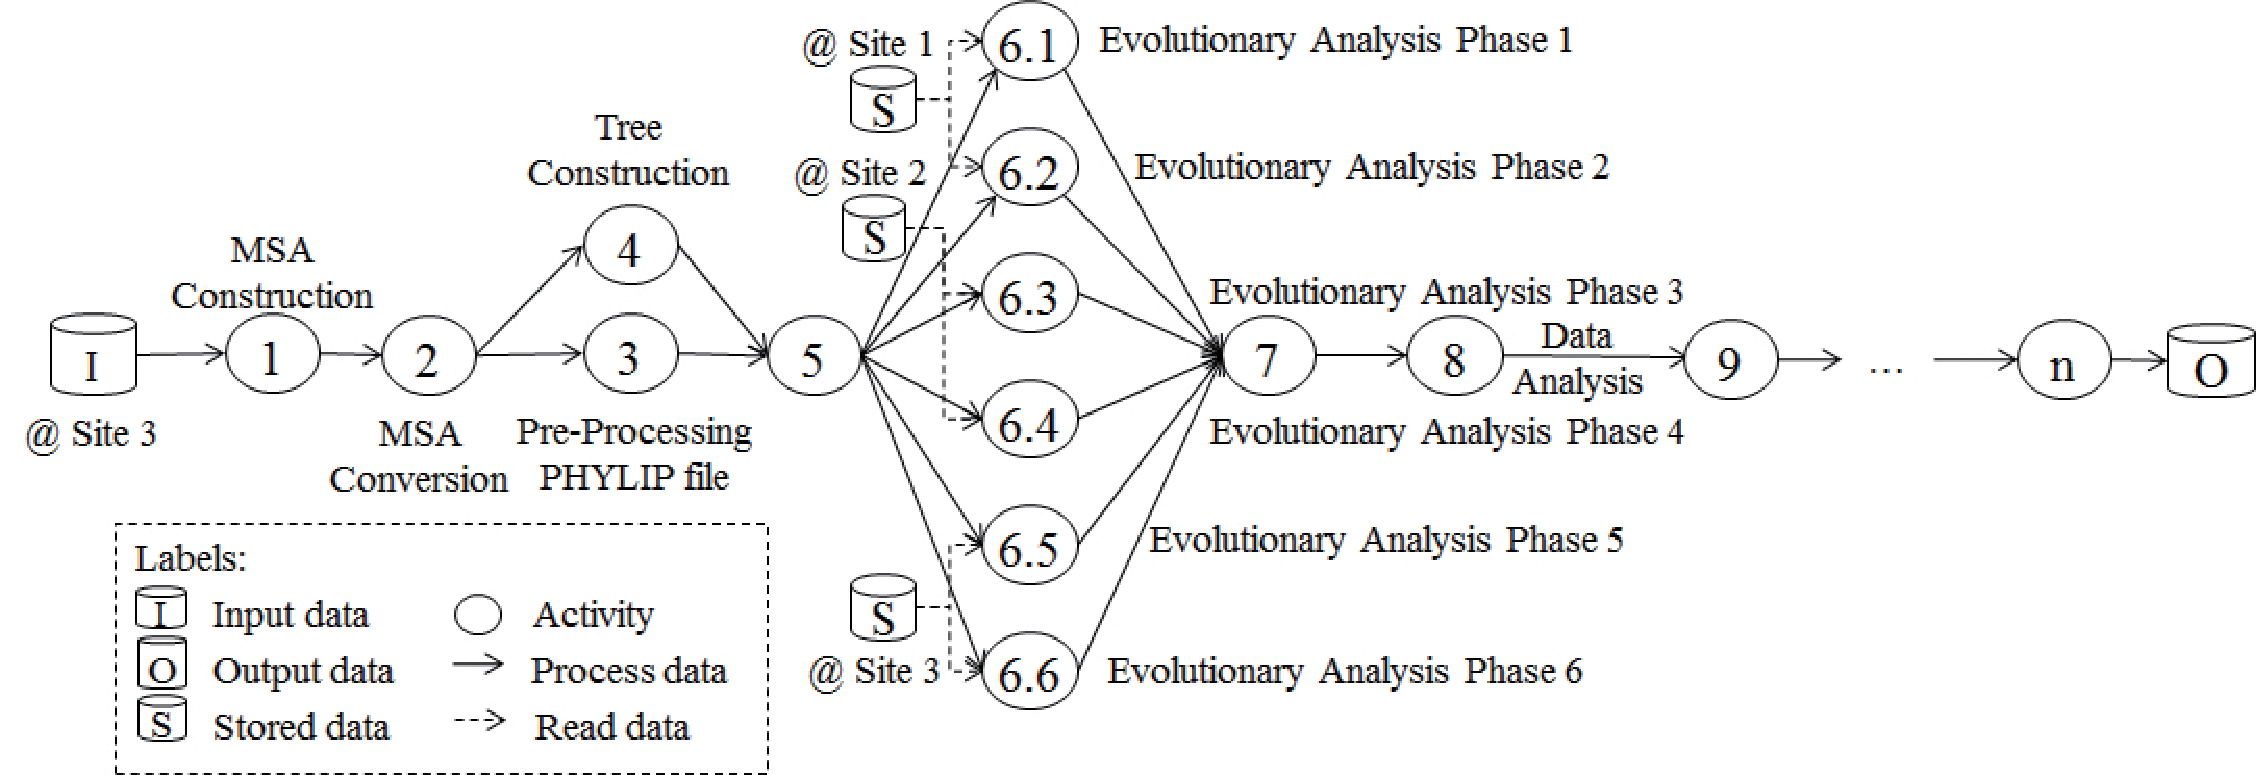
\includegraphics[width=140mm]{figures/FIG16}
\par\end{centering}
\caption{\textbf{SciEvol SWf. } Activities $9 - n$  are added control activities, which have no workload.}
\label{fig:nscievol}
\end{figure*}


\begin{table*}[htbp]
\caption{\textbf{Number of generations. }}
\label{tab:generations}
\begin{centering}
\captionsetup{justification=centering}
\begin{tabular}{|c|c|c|c|c|c|c|c|c|c|c|c|}
\cline{1-10}
Number of sites & 3 & 4 & 5 & 6 & 7 & 8 & 9 & 10 & 11 \\
\cline{1-10}  
Number of generations & 1 & 1 & 3 & 10 & 28 & 71 & 162 & 337 & 657 \tabularnewline
\cline{1-10}
\hline
Number of activities & 13 & 14 & 15 & 16 & 17 & 18 & 19 & 20 & 21 & 22 & 23 \\
\hline  
Number of generations & 1 & 1 & 1 & 2 & 6 & 18 & 54 & 162 & 484 & 1450 & 4349 \tabularnewline
\hline
\end{tabular}
\par\end{centering} 
\end{table*}

An example of scheduling time corresponding to $3$ sites and $13$ activities is shown in Table \ref{tab:MST}. This is a small example since the time necessary to schedule the activities may be unfeasible for Brute-force and Genetic when the numbers of activities or sites become high. Then, we vary the numbers of activities or sites. When we increase the number of sites, we fix the number of activities at $13$ and when we increase the number of activities, we fix the number of sites to $3$. The number of generations for different numbers of activities or different numbers of sites is shown in Table \ref{tab:generations}. Since the search space gets bigger when the number of activities or sites increases, we increase the number of generations in order to evaluate at least $30\%$ of all the possible scheduling plans for Genetic. We add additional control activities in the SciEvol SWf, which have little workload but increase the search space of scheduling plans. The modified SciEvol SWf is shown in Figure \ref{fig:nscievol} and the scheduling time corresponding to different numbers of activities is shown in \ref{fig:an}. In addition, we measure the scheduling time corresponding to different numbers of sites while using the original SciEvol SWf, as shown in Figure \ref{fig:sn}. 
The unit of scheduling time is millisecond.
The data constraint remains the same while the number of input files is $100$ and $\alpha$ equals to $0.9$. In the experiments, only ActGreedy generates the same scheduling plans as that of Brute-force. Since the point of mutation operation and the points of crossover operation of Genetic are randomly selected, the scheduling plans generated by Genetic may not be stable, \textit{i.e.} the scheduling plans may not be the same for each execution of the algorithm. Both LocBased and SGreedy cannot generate the optimal scheduling plans as that of Brute-force.

\begin{table}[htbp]
\caption{\textbf{Comparison of scheduling algorithms. }}
\label{tab:MST}
\begin{centering}
\captionsetup{justification=centering}
\begin{tabular}{|c|c|c|c|c|c|}
\hline
Algorithms & Scheduling time (ms) \tabularnewline
\hline
LocBased & 0.010 \tabularnewline
\hline
SGreedy & 0.014 \tabularnewline
\hline
ActGreedy & 1.260 \tabularnewline
\hline
Genetic & 727 \tabularnewline
\hline
Brute-force & 161 \tabularnewline
\hline
\end{tabular}
\par\end{centering}
\end{table}

Table \ref{tab:MST} shows that the scheduling time of Genetic and Brute-force is much longer than ActGreedy (up to $577$ times and $128$ times). Genetic may perform worse than Brute-force for a small number of activities or sites with the specific configuration. The schedul-
\begin{figure*}
\begin{centering}
		\subfigure[\textbf{Scheduling time corresponding to different numbers of activities.}]{\includegraphics[width=59mm]{figures/FIG17_1} \label{fig:an}} 
		\subfigure[\textbf{Scheduling time corresponding to different numbers of sites.} ]{\includegraphics[width=59mm]{figures/FIG17_3} \label{fig:sn}} 
		\subfigure[\textbf{Scheduling time corresponding to different numbers of activities (zoom on LocBased, SGreedy and ActGreedy).}]{\includegraphics[width=59mm]{figures/za} \label{fig:za}} 
		\subfigure[\textbf{Scheduling time corresponding to different numbers of sites (zoom on LocBased, SGreedy and ActGreedy).} ]{\includegraphics[width=59mm]{figures/zs} \label{fig:zs}} 
\caption{\textbf{Scheduling time.} }\label{fig:ST}
\end{centering}
\end{figure*}
\noindent ing time of Genetic is smaller than that of Brute-force when the number of activities or sites increases as shown in Figure \ref{fig:an} and \ref{fig:sn}. 
Figures \ref{fig:an} and \ref{fig:sn} show that the scheduling time of ActGreedy, SGreedy and LocBased is much smaller than that of Genetic and Brute-force. The scheduling time of ActGreedy, SGreedy and LocBased is represented by the bottom line in Figures \ref{fig:an}\ref{fig:sn}. Even though when the number of activities and the number of sites is small, the scheduling time is negligible compared with the execution time, it becomes significant when the numbers of activities or sites increase. For instance, with more than $22$ activities or $6$ sites, the scheduling time of Brute-force exceeds the execution while the scheduling time of ActGreedy remains small. This is because of the high complexity of Brute-force, which is $\mathcal{O}(s ^ { n - f })$. With more than $22$ activities or $10$ sites, the scheduling time of Genetic is bigger than the execution time. Because of long scheduling time, Genetic and Brute-force are not suitable for SWfs with a big number of activities, \textit{e.g.} Montage \cite{Montage} may have $77$ activities. In addition, according to \cite{Littauer2012}, $22$ activities are below the average number of SWf activities. As a result, Genetic and Brute-force are unfeasible for multisite scheduling of most SWfs. These two algorithms are not suitable for SWf scheduling with a big number of sites. For instance, Azure has $15$ sites (regions). Although the scheduling time of ActGreedy is much bigger (see Figures \ref{fig:za}\ref{fig:zs} for details) than that of SGreedy and LocBased, it remains reasonable compared with the overall SWf execution time. 

The experimental results show that although ActGreedy may yield more data transferred among different sites and higher idleness (compared with LocBased), it generally yields smaller cost compared with both LocBased and SGreedy and the scheduling time of ActGreedy is much lower than that of Genetic and Brute-force.

\section{Conclusion}
\label{sec:Con}

Scientists usually make intensive usage of parallelism techniques in HPC environments.  However, it is not simple to schedule and manage executions of SWfs, particularly in multisite cloud environments, which present different characteristics in comparison with a single site cloud. To increase the uptake  of the cloud model for executing SWfs that demand HPC capabilities provided by a multisite cloud and to benefit from data locality, new  solutions have to be developed,  especially for scheduling SWf fragments in cloud resources. In previous work \cite{Oliveira2012} we have addressed SWf execution in a single site cloud using a scheduling algorithm but these solutions are not suitable for a multisite cloud.

In this chapter, we proposed a new multi-objective scheduling approach, \textit{i.e.} ActGreedy, for SWfs in a multisite cloud (from the same provider). We first proposed a novel multi-objective cost model, which aims at minimizing two costs: execution time and monetary costs.
Our proposed fragment scheduling approach that is ActGreedy, allows for considering stored data constraints while reducing the cost based on the multi-objective cost model to execute a SWf in a multisite cloud. 
We used a real SWf that is SciEvol, with real data from the bioinformatics domain as a use case. We evaluated our approaches by executing SciEvol in Microsoft Azure cloud. The results show that since ActGreedy makes a good trade-off between execution time and monetary costs, ActGreedy leads to the least total normalized cost, which is calculated based on the multi-objective cost model, than LocBased (up to $10.7\%$) and SGreedy (up to $17.2\%$) approaches. 
In addition, compared with LocBased (up to $14.12\%$) and SGreedy (up to $17.28\%$), ActGreedy always corresponds to less monetary cost since it can choose cheap cloud sites to execute SWf fragments.
Furthermore, compared with SGreedy, ActGreedy corresponds to more than two times smaller amounts of transferred data. 
Additionally, ActGreedy scales very well, \textit{i.e.} it takes a very small time to generate the optimal or near optimal scheduling plans when the number of activities or sites increases, compared with general approaches, \textit{e.g.} Genetic and Brute-force.